\chapter{Experimental Results}
\label{chapter:experimentalresults}
This chapter will introduce the actual experiments we have conducted in this project. It will first discuss the performance benefits of the different optimization techniques we have used and generalize with the speed-ups achieved over the sequential set-up we have discussed in chapter~\ref{chapter:sequential}. The chapter will conclude with a summary of our findings aiming to answer the thesis questions stated in the beginning of the report. 

As mentioned in the previous chapter, we ran our 5 programs on 7 datasets with many combinations of parameters such as version, sorting and block size, which gave us a large number of results (3542 in total). Therefore, it is important to show only the results that matter the most, and we decided to make plots that show the best runtimes and average memory we measured for the combination shown on the plot.
Even though we have created a variety of plots to support our findings, in this chapter we will only show the ones which can clearly show the differences we discuss. Since we have distributions of different nature, we expect to see opposing differences for some optimizations. Therefore, to underline the trade-offs and the importance of each optimization, we have tried to show on plots the two datasets that have shown the most contrast in each experiment. Nevertheless, all results can be found in tables under the two chosen plots and all plots can be found in Appendices B, C and D.

\section{CUDA-option Performance}
\subsection{Coalescing}
As it can be seen on fig.~\ref{fig:experiments:cudaoption:versions}, coalescing (versions 2, 3 and 4 all provide memory coalescing) has proven to be a successful technique for \textit{CUDA-option}. The highest performance was achieved on the random dataset with constant height, where we have achieved as much speed-up as \textasciitilde$10\times$ on floats and \textasciitilde$2\times$ on doubles. The least impact by coalescing has shown to be on the skewed datasets, even though still \textasciitilde$2\times$ faster. 

\begin{figure}[H]
\centering
\begin{subfigure}{.49\textwidth}
  \centering
  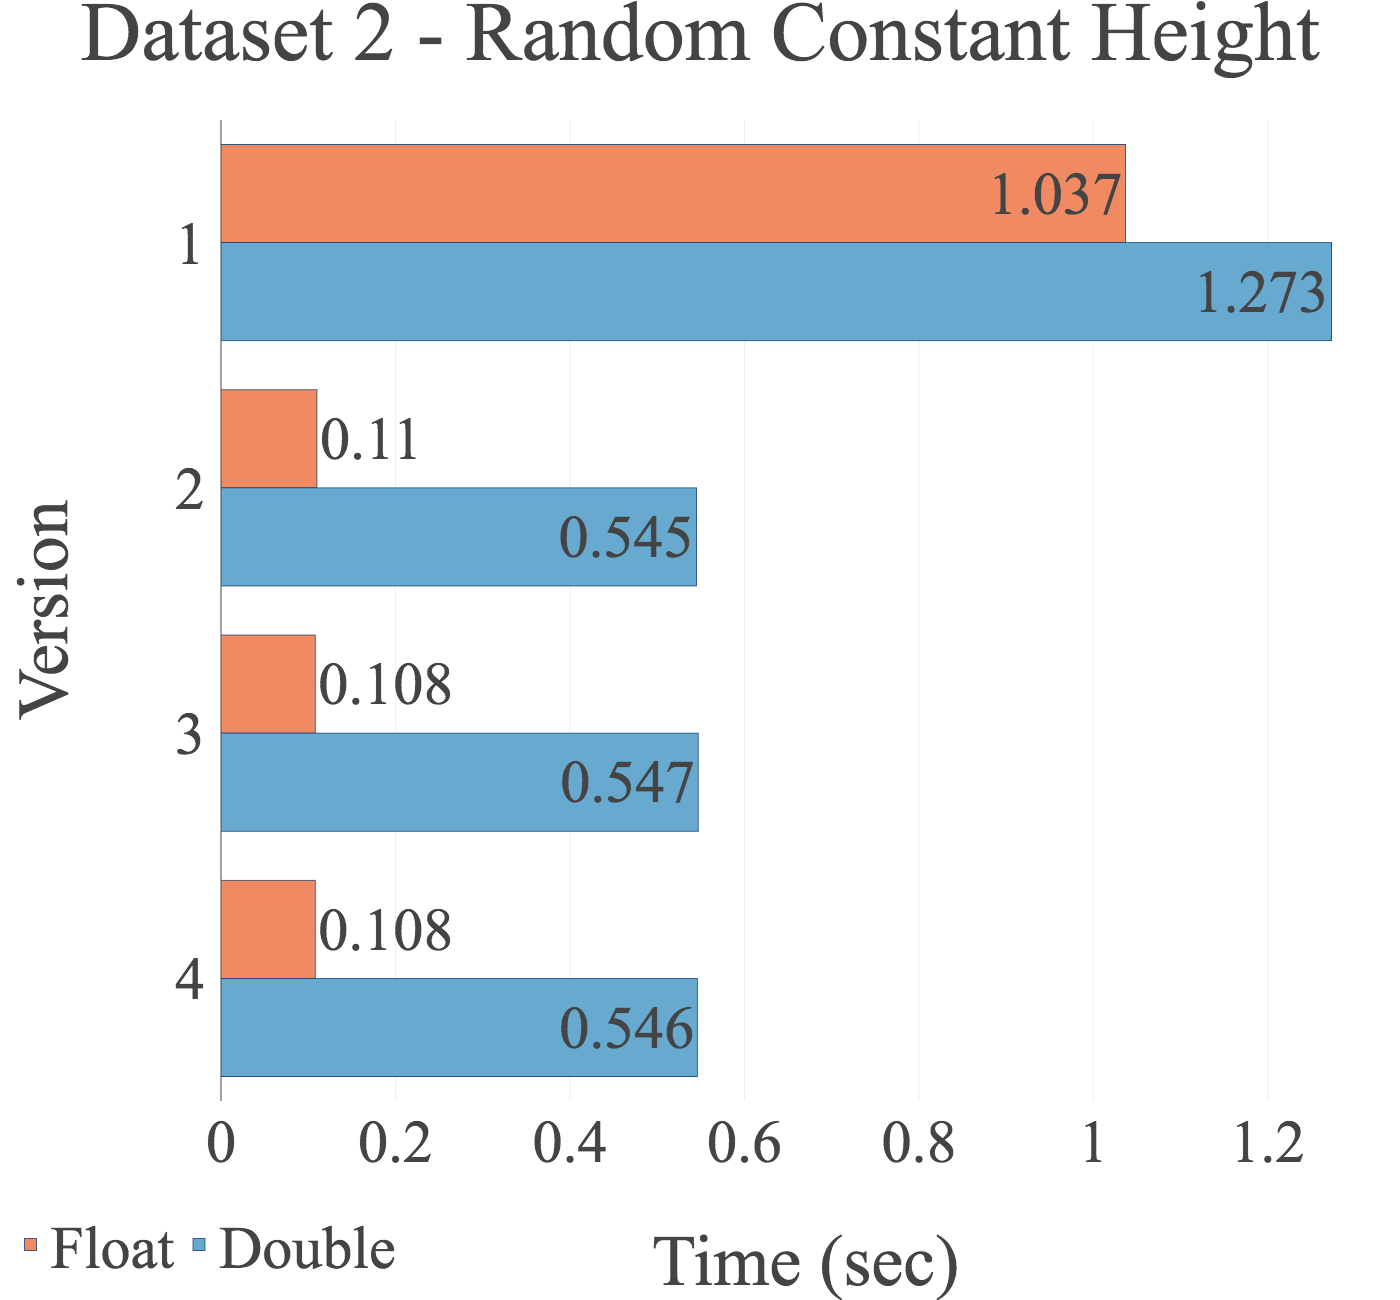
\includegraphics[width=1\linewidth]{img/experiments/option-versions-2_RANDCONSTHEIGHT.png}
\end{subfigure}
\begin{subfigure}{.49\textwidth}
  \centering
  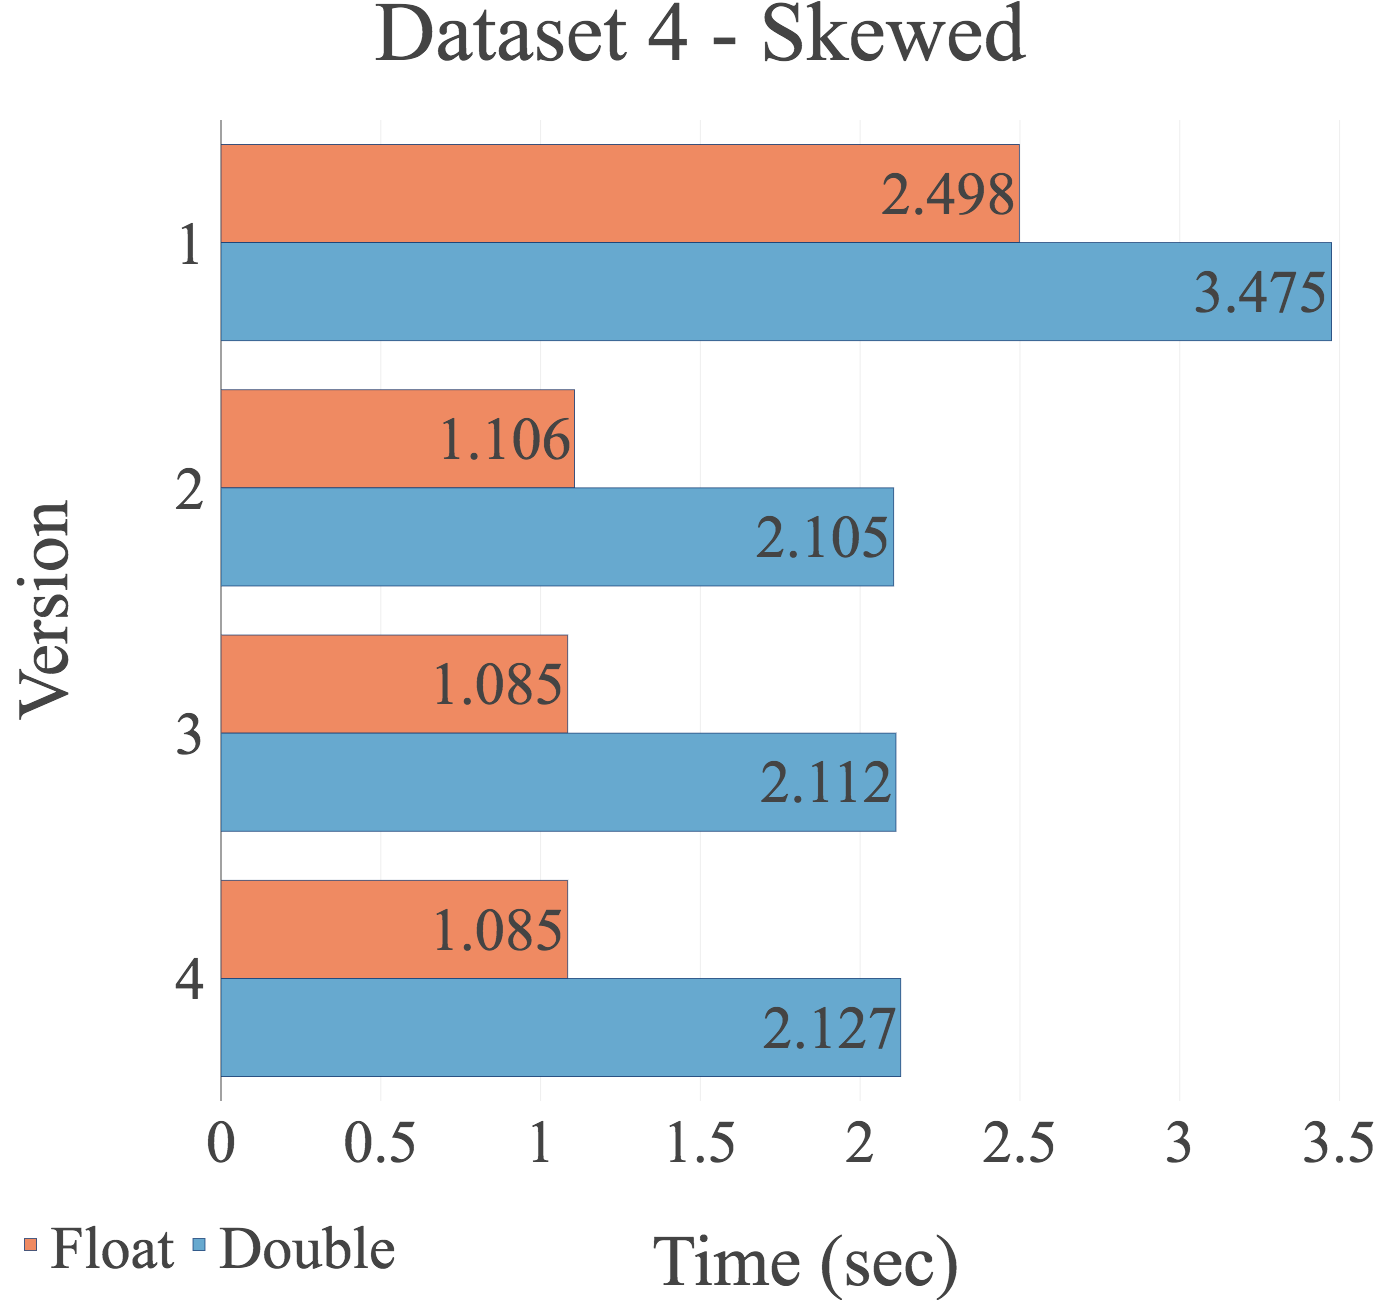
\includegraphics[width=1\linewidth]{img/experiments/option-versions-4_SKEWED.png}
\end{subfigure}
\begin{center}
  \small
  \captionof{table}{Float runtime for all 7 datasets (in seconds)}
  \csvautotabular{csv/option-versions-float.csv}
\end{center}
\begin{center}
  \small
  \captionof{table}{Double runtime for all 7 datasets (in seconds)}
  \csvautotabular{csv/option-versions-double.csv}
\end{center}
\caption{Performance impact of coalescing in \textit{CUDA-option} (best runtimes)}
\label{fig:experiments:cudaoption:versions}
\end{figure}

\newpage
\subsection{Global-level Padding}
While the runtime improvements were significant after the coalescing, memory consumption had also increased with the usage of global-level padding in version 2 (up to \textasciitilde$7\times$ more for both floats and doubles), in comparison to version 1. This can be seen on fig.~\ref{fig:experiments:cudaoption:memory} showing the memory consumption difference between all versions for datasets 1 - Random and 4 - Skewed. This was obviously unwanted and it was therefore necessary to try and reduce the memory usage.

\subsection{Block-level Padding}
As described in chapter~\ref{chapter:oneoptionperthread}, block-level padding (version 3) is a memory optimization technique, which attempts to reduce the large memory usage, while preserving coalesced memory access. This version has proven to significantly reduce memory size, as it can be seen on fig.~\ref{fig:experiments:cudaoption:memory}, while the performance remained similar. On average, requiring \textasciitilde$1.4\times$ less memory than version 2 for floats and \textasciitilde$3\times$ for doubles, but still \textasciitilde$2\times$ more than version 1.

\subsection{Warp-level Padding}
Warp-level padding (version 4) was also described in chapter~\ref{chapter:oneoptionperthread}, where arrays were padded per 32 threads (warp) instead of a block, compared to version 3. On average, it used \textasciitilde$1.4\times$ less memory than block-level padding, bringing it down to \textasciitilde$1.4\times$ more memory than no padding (fig.~\ref{fig:experiments:cudaoption:memory}), while performance remained similar again (fig.~\ref{fig:experiments:cudaoption:versions}).

\begin{figure}[H]
\centering
\begin{subfigure}{.49\textwidth}
  \centering
  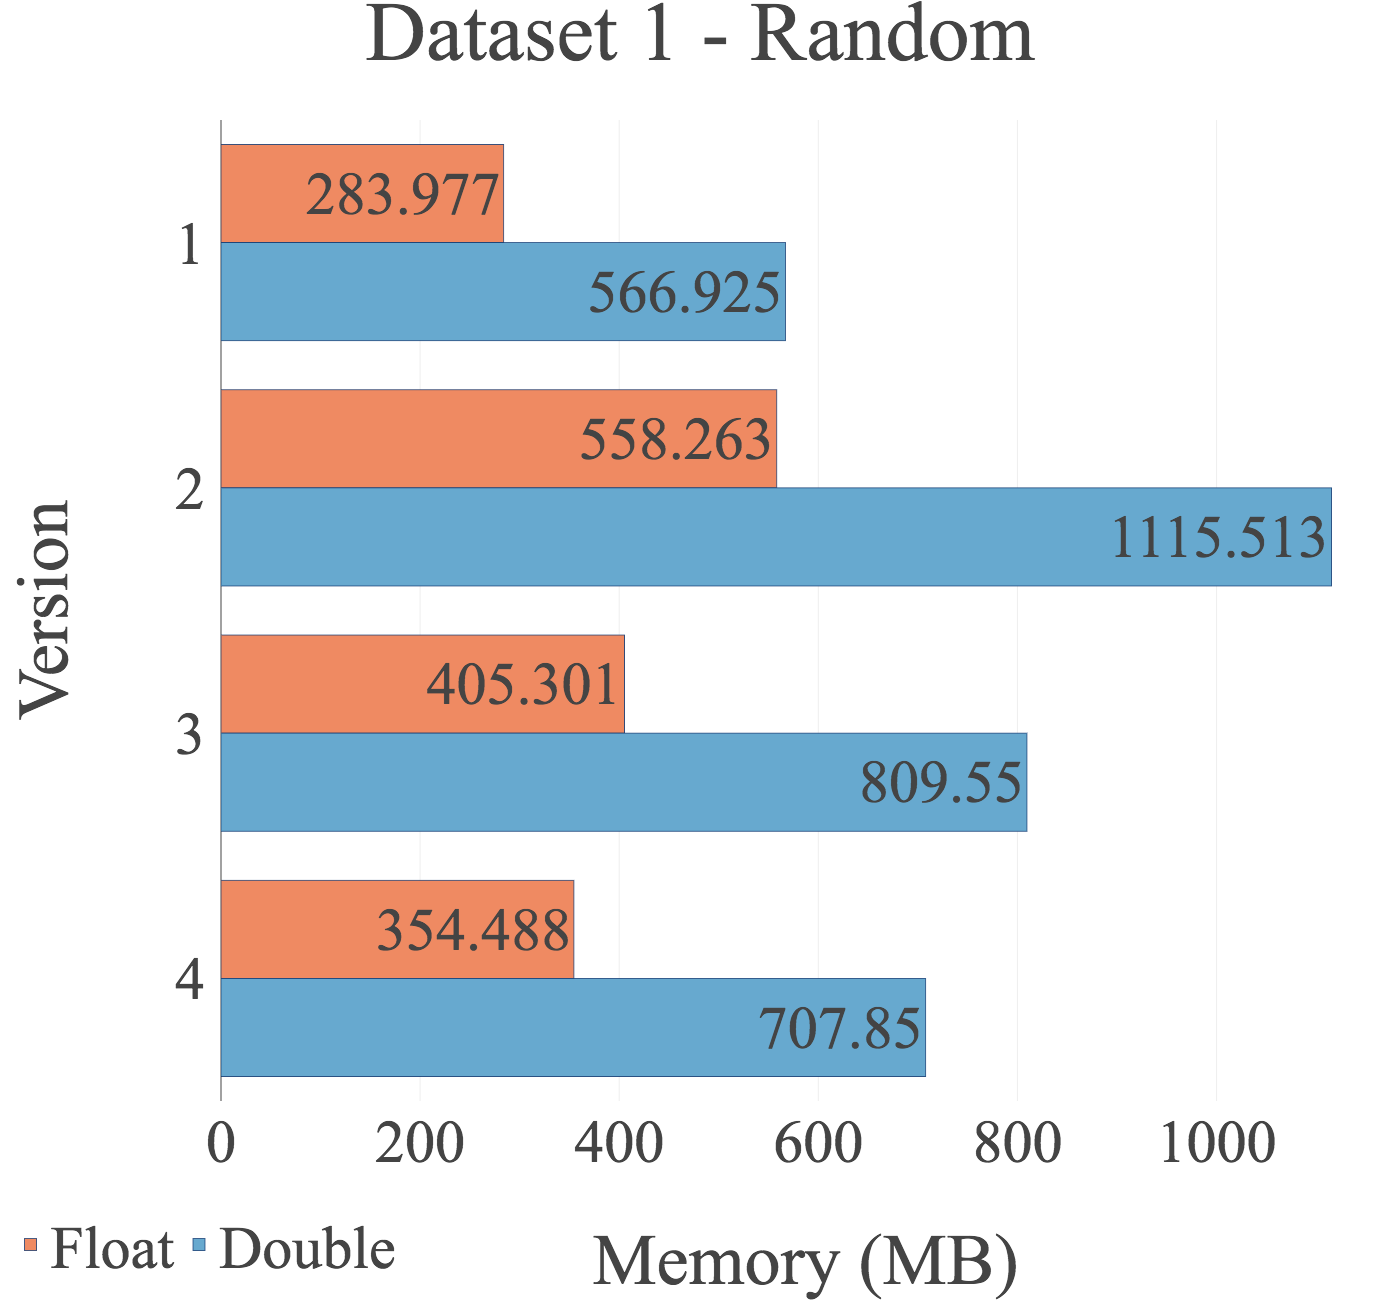
\includegraphics[width=1\linewidth]{img/experiments/mem-option-versions-1_RAND.png}
\end{subfigure}
\begin{subfigure}{.49\textwidth}
  \centering
  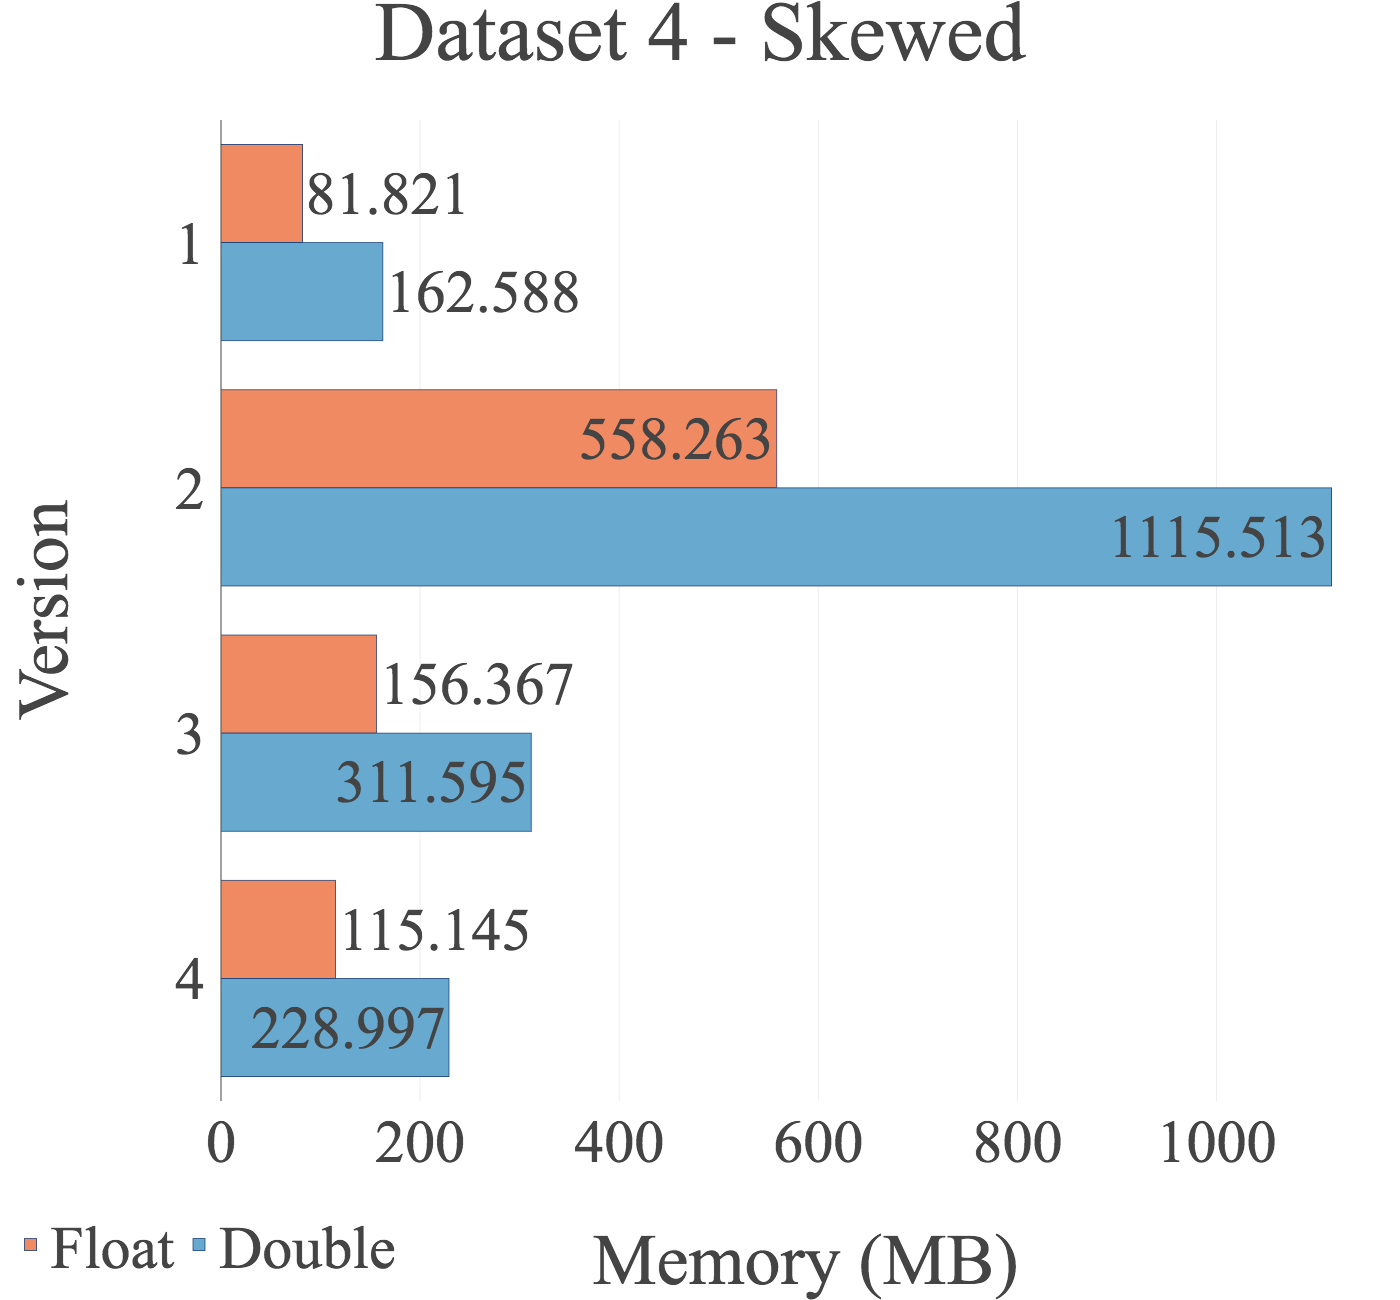
\includegraphics[width=1\linewidth]{img/experiments/mem-option-versions-4_SKEWED.png}
\end{subfigure}
\begin{center}
  \small
  \captionof{table}{Float memory size for all 7 datasets (in MB)}
  \csvautotabular{csv/mem-option-versions-float.csv}
\end{center}
\begin{center}
  \small
  \captionof{table}{Double memory size for all 7 datasets (in MB)}
  \csvautotabular{csv/mem-option-versions-double.csv}
\end{center}
\caption{Memory impact of padding in \textit{CUDA-option} (average global memory size)}
\label{fig:experiments:cudaoption:memory}
\end{figure}

\newpage
\subsection{Sorting}
\label{section:sortingcudaoption}
An important optimization technique which affects thread divergence is sorting. We tested 4 types of sorting:
\begin{enumerate}
    \item ascending height first, width second
    \item descending height first, width second
    \item ascending width first, height second
    \item descending width first, height second
\end{enumerate}

As shown on fig.~\ref{fig:experiments:cudaoption:sorting}, dataset 0 - Uniform data distribution, is negatively affected by it, as we also have to spend a few milliseconds to sort the data and gain no actual benefit for doing that. This is expected, since all options in the file have the exact same width and height. We expect, however, that sorting similar data distributions, where the distribution of data is centered around the middle (similar to fig.~\ref{fig:experimentmethodology:uniform} but not just one point), can lead to a small, insignificant speed-up. Hence the only situation where we found sorting useless was when pricing a large number of duplicated options, which is impractical.  

In contrast, sorting has proven to be quite successful on other datasets. However, as mentioned in chapter~\ref{chapter:oneoptionperthread}, and shown on fig.~\ref{fig:experiments:cudaoption:sorting}, choosing a good sorting strategy can be data-sensitive. We can see on the plot for dataset 5 - Skewed constant height that any sorting is better than no sorting at all. Despite that, different sorting options can produce different speed-ups with up to 20\% of margin.

Due to the thread divergence, we risk running large options (e.g. options with large heights) in the end, which likely results in CUDA waiting on a few threads to process them, while a lot of other threads are idling. Intuitively, reducing the idle time for threads can produce significant speed-ups, hence we expect that sorting by descending should be generally better in most cases. Looking at the additional plots in Appendix \ref{appendix:option:sorting} or tables in fig.~\ref{fig:experiments:cudaoption:sorting}, we can confirm our observation, as sorting by both width and height in descending order tends to be faster. 

Additionally, we show that pre-processing (primarily affected by sorting) takes a negligible amount of time in all cases, as seen in fig.~\ref{fig:experiments:cudaoption:sorting-prep}, where the highest average pre-processing time for doubles takes 12.3 milliseconds when sorting by ascending width. 

\begin{figure}[H]
\centering
\begin{subfigure}{.49\textwidth}
  \centering
  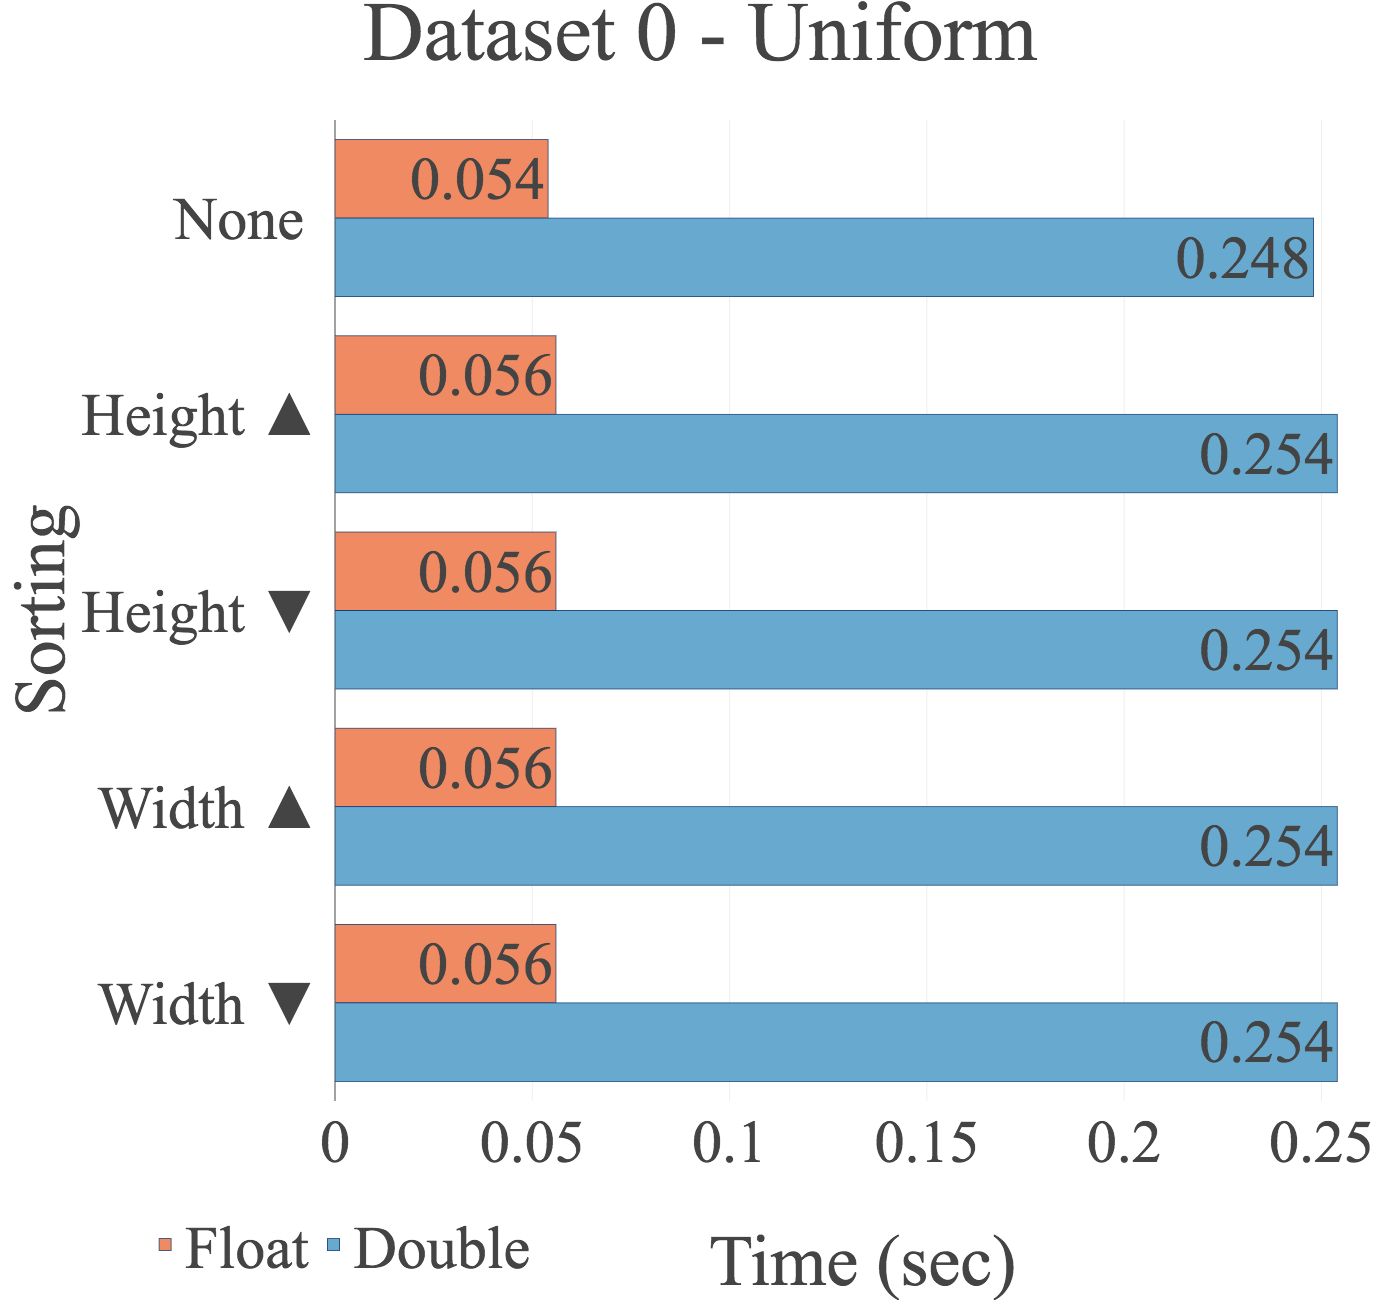
\includegraphics[width=1\linewidth]{img/experiments/option-sorts-0_UNIFORM.png}
\end{subfigure}
\begin{subfigure}{.49\textwidth}
  \centering
  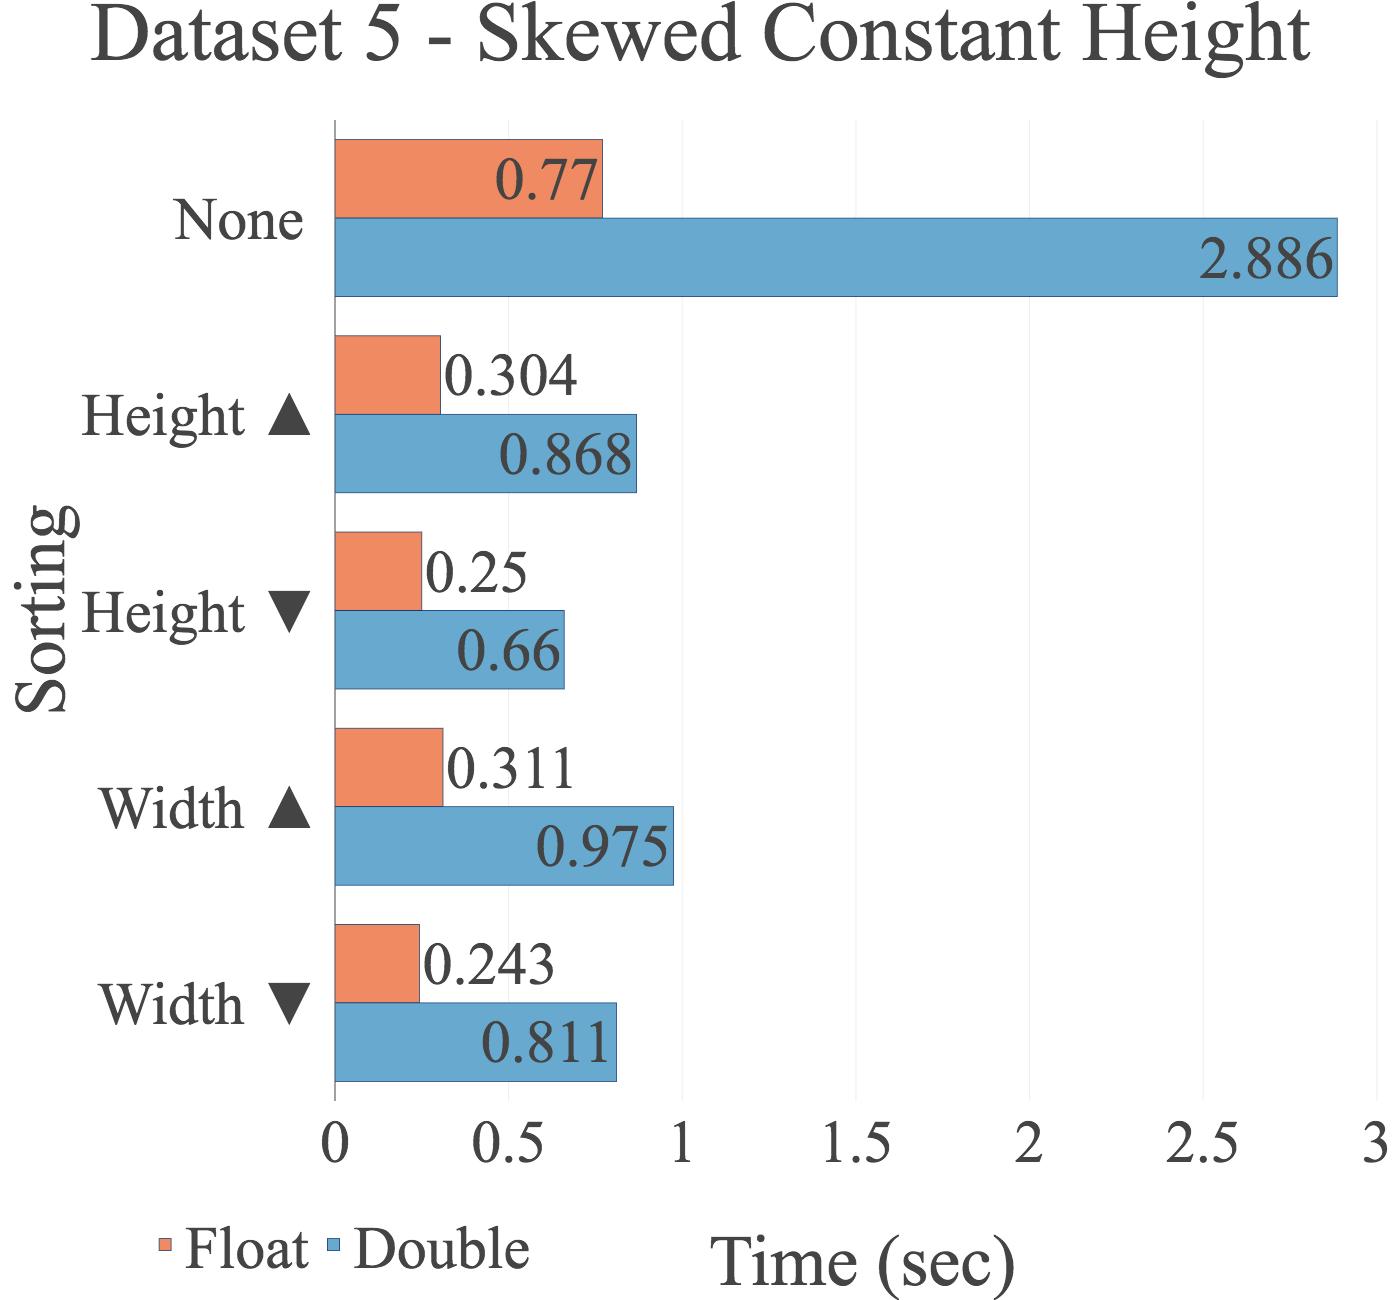
\includegraphics[width=1\linewidth]{img/experiments/option-sorts-5_SKEWEDCONSTHEIGHT.png}
\end{subfigure}
\begin{center}
  \small
  \captionof{table}{Float runtime for all 7 datasets (in seconds)}
  \csvautotabular{csv/option-sorts-float.csv}
\end{center}
\begin{center}
  \small
  \captionof{table}{Double runtime for all 7 datasets (in seconds)}
  \csvautotabular{csv/option-sorts-double.csv}
\end{center}
\caption{Performance impact of sorting in \textit{CUDA-option} (best runtimes)}
\label{fig:experiments:cudaoption:sorting}
\end{figure}

\begin{figure}[H]
\begin{center}
  \small
  \captionof{table}{Float pre-processing time for all 7 datasets (in \textbf{milliseconds})}
  \csvautotabular{csv/option-sorts-prep-float.csv}
  \label{table:experiments:cudaoption:sortingcostfloats}
\end{center}
\begin{center}
  \small
  \captionof{table}{Double pre-processing time for all 7 datasets (in \textbf{milliseconds})}
  \csvautotabular{csv/option-sorts-prep-double.csv}
  \label{table:experiments:cudaoption:sortingcostdoubles}
\end{center}
\caption{Pre-processing cost in \textit{CUDA-option} (average pre-processing times)}
\label{fig:experiments:cudaoption:sorting-prep}
\end{figure}

\subsection{Block Sizes}
Since \textit{CUDA-option} is concerned with running a single option per thread, the block size determines the number of options that can be processed in parallel. This was also described at the end of chapter~\ref{chapter:oneoptionperthread}, together with an explanation of the trade-offs for choosing different block sizes. The two experiments we have chosen to display in this section (see fig.~\ref{fig:experiments:cudaoption:blocks}) show that the optimal block-size is also dependent on the data. Even though the impact of block sizes is not significant (i.e. \textasciitilde$1.5\times$ for floats and \textasciitilde$1.2\times$ for doubles), dataset 1 - Random performs best with a block size of 128. In contrast, dataset 5 - Skewed Constant Height operates best with block size of 512. Despite that, smaller block sizes prevail to show optimal performance on all other experiments (as seen in Appendix~\ref{appendix:option:block} or tables in fig.~\ref{fig:experiments:cudaoption:blocks}).

\begin{figure}[H]
\centering
\begin{subfigure}{.49\textwidth}
  \centering
  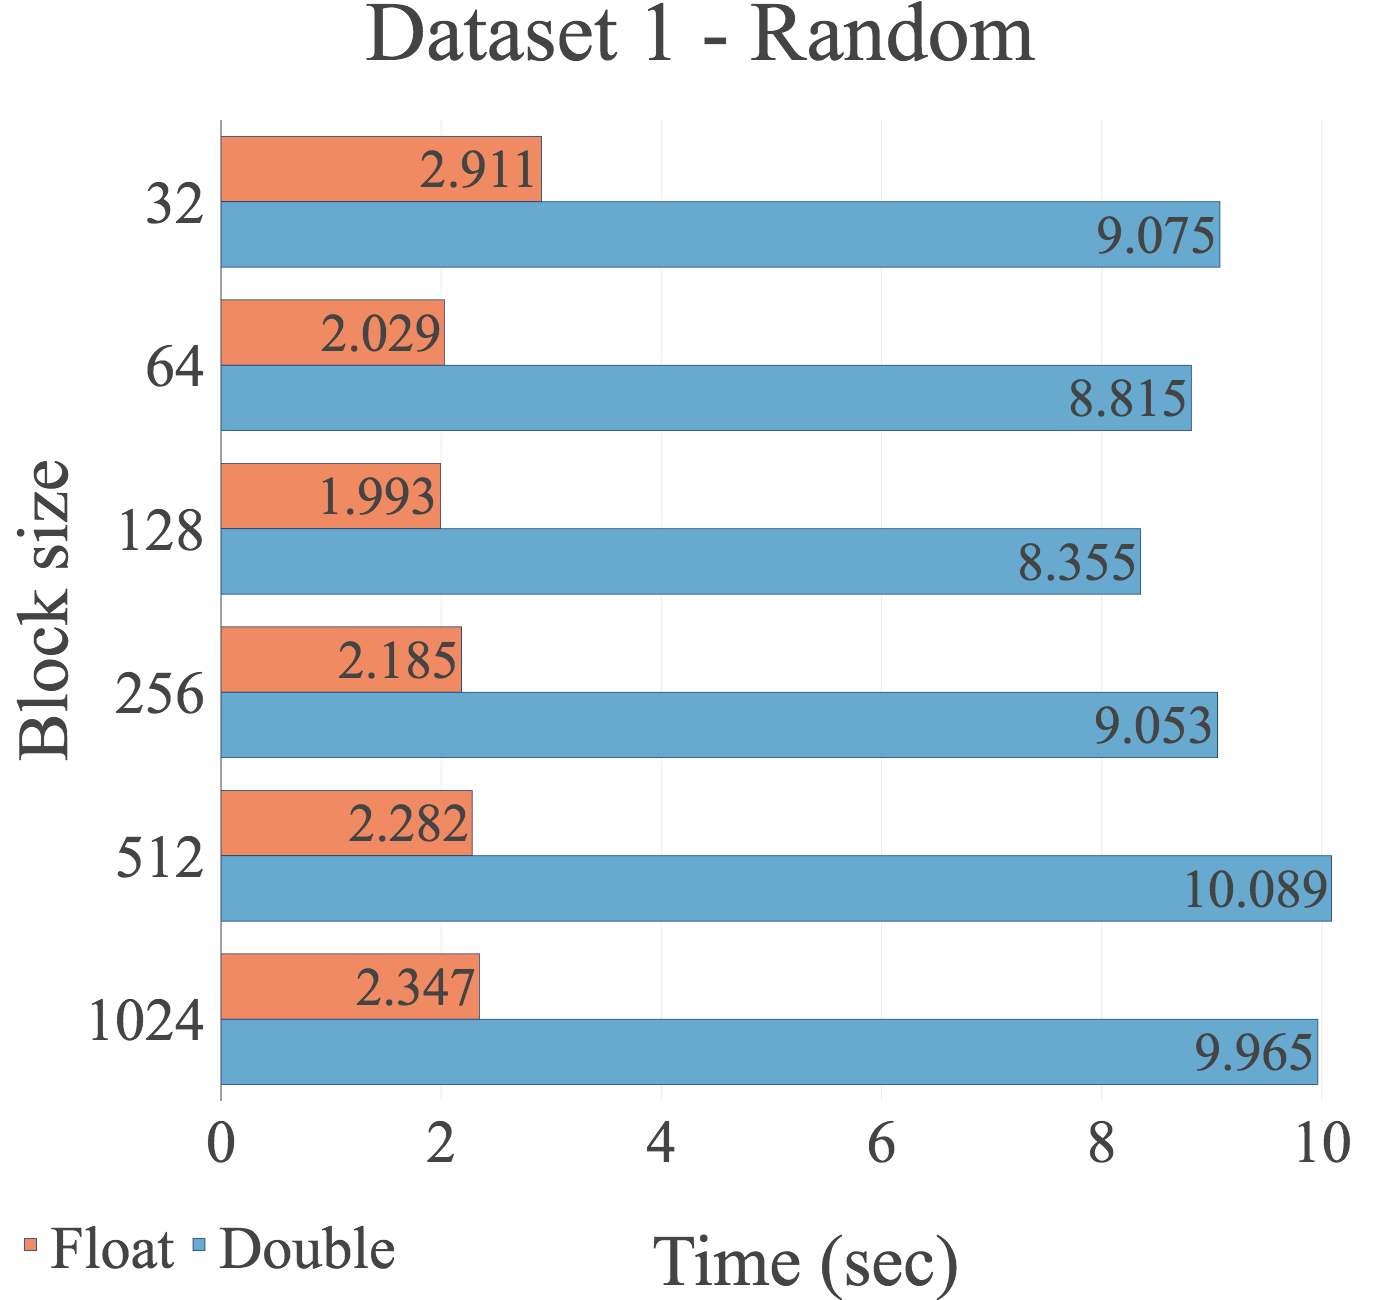
\includegraphics[width=1\linewidth]{img/experiments/option-blocks-1_RAND.png}
\end{subfigure}
\begin{subfigure}{.49\textwidth}
  \centering
  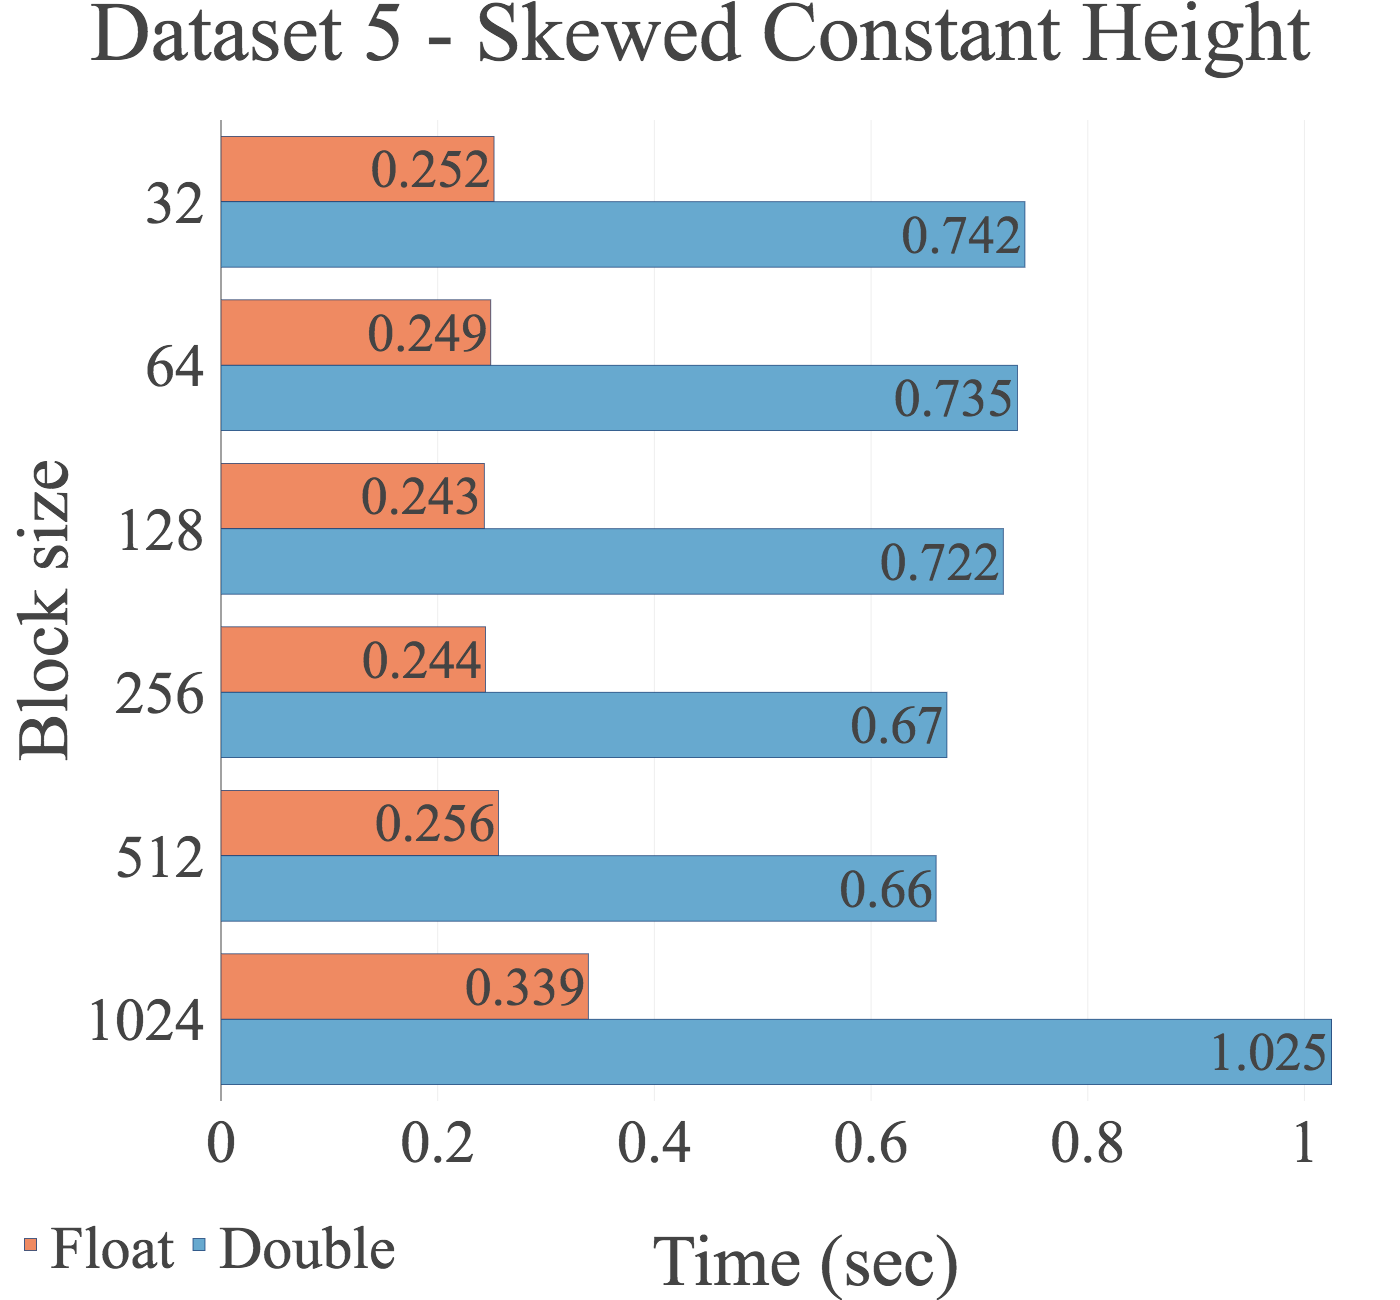
\includegraphics[width=1\linewidth]{img/experiments/option-blocks-5_SKEWEDCONSTHEIGHT.png}
\end{subfigure}
\begin{center}
  \small
  \captionof{table}{Float runtime for all 7 datasets (in seconds)}
  \csvautotabular{csv/option-blocks-float.csv}
\end{center}
\begin{center}
  \small
  \captionof{table}{Double runtime for all 7 datasets (in seconds)}
  \csvautotabular{csv/option-blocks-double.csv}
\end{center}
\caption{Performance impact of different block sizes in \textit{CUDA-option} (best runtimes)}
\label{fig:experiments:cudaoption:blocks}
\end{figure}

\section{CUDA-multi performance}
\subsection{Coalescing}
Both version 1 and version 2 of \textit{CUDA-multi} use global-level padding to allocate height-dependent arrays (alphas). Their difference comes in the memory coalescing. Interestingly enough, all experiments we have created to test the performance benefits of coalescing on \textit{CUDA-multi} have shown no significant improvement. This can be seen on fig.~\ref{fig:experiments:cudamulti:coalescing}. The only reasonable explanation for this is that \textit{CUDA-multi} does not access that many alphas at the same time. For example, in \textit{CUDA-option} on a uniform dataset, using a block size of 1024 will make all 1024 threads access alphas at the same time, which makes it easy to optimize data transfers by coalescing. On the other hand, in \textit{CUDA-multi} the number of alphas accessed at the same time depends primarily on the number of options in the block and their widths. Nevertheless, this number is going to be much smaller, making optimizations much less significant.

\begin{figure}[H]
\centering
\begin{subfigure}{.49\textwidth}
  \centering
  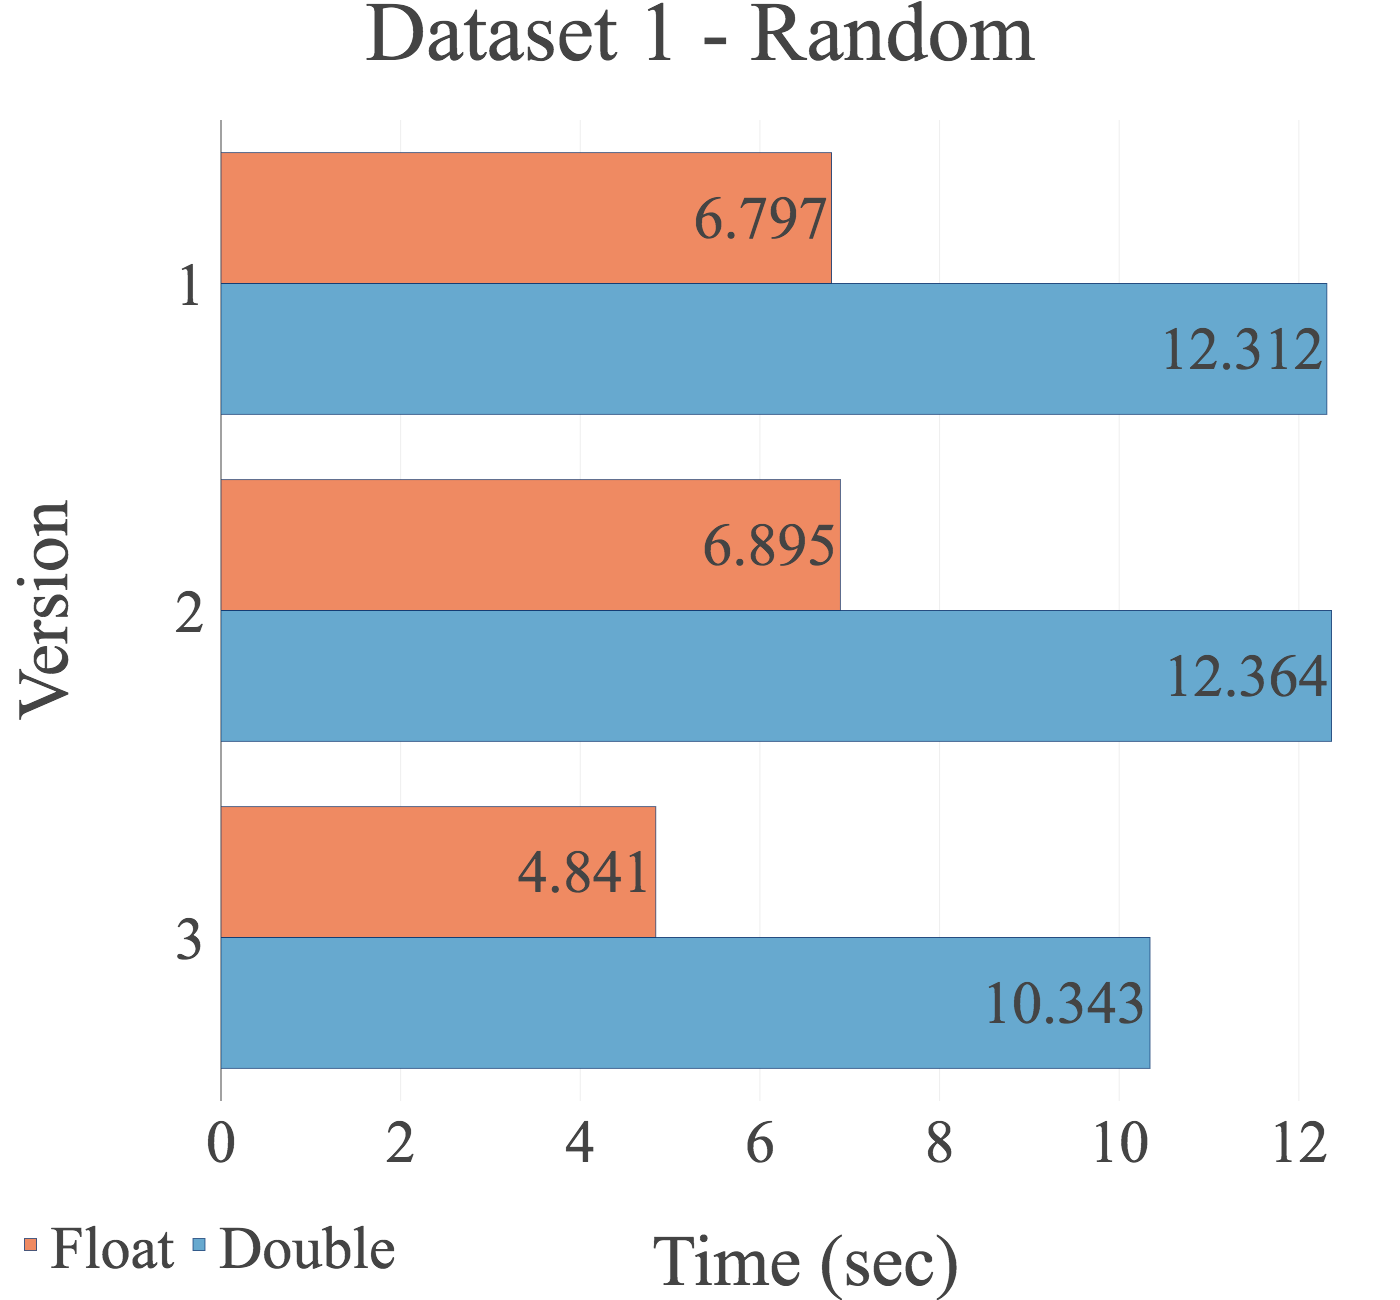
\includegraphics[width=1\linewidth]{img/experiments/multi-versions-1_RAND.png}
\end{subfigure}
\begin{subfigure}{.49\textwidth}
  \centering
  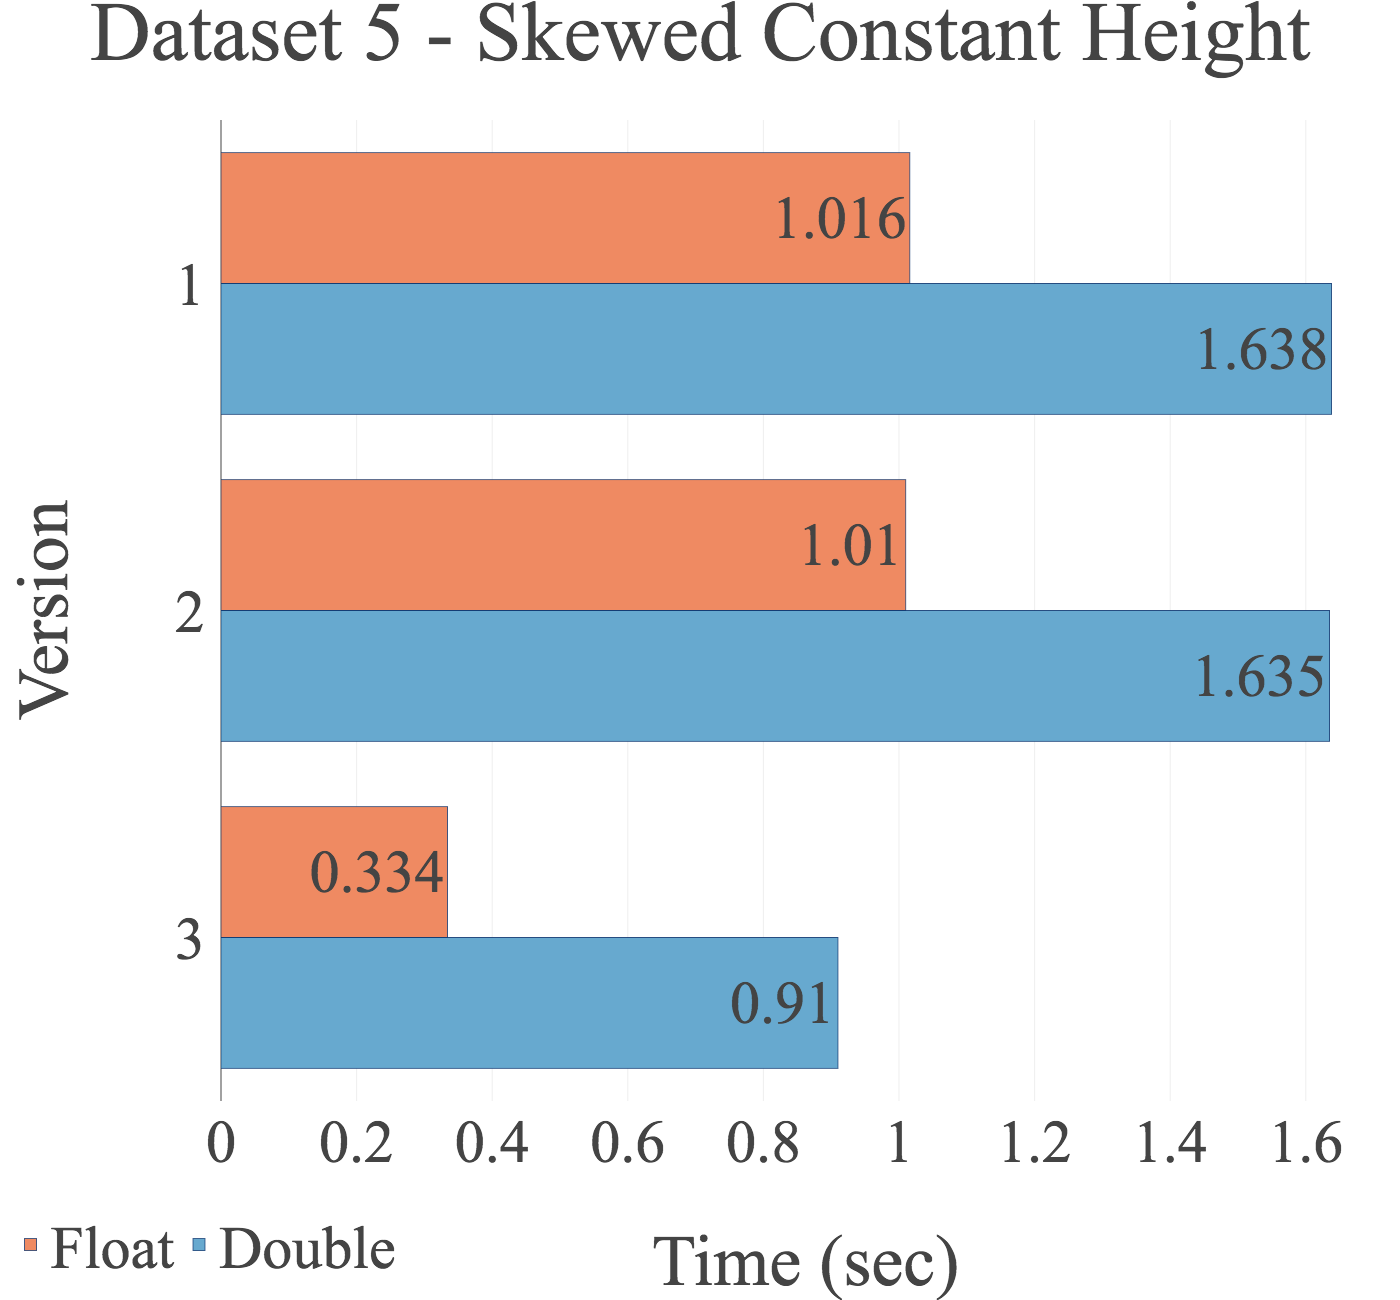
\includegraphics[width=1\linewidth]{img/experiments/multi-versions-5_SKEWEDCONSTHEIGHT.png}
\end{subfigure}
\begin{center}
  \small
  \captionof{table}{Float runtime for all 7 datasets (in seconds)}
  \csvautotabular{csv/multi-versions-float.csv}
\end{center}
\begin{center}
  \small
  \captionof{table}{Double runtime for all 7 datasets (in seconds)}
  \csvautotabular{csv/multi-versions-double.csv}
\end{center}
\caption{Performance impact of memory coalescing on \textit{CUDA-multi} (best runtimes)}
\label{fig:experiments:cudamulti:coalescing}
\end{figure}

\newpage
\subsection{Global-level Padding}
As noted in the previous section, both version 1 and 2 use global-level padding and no memory-optimizing technique has been applied. Hence we do not expect any memory differences between the two. Fig.~\ref{fig:experiments:cudamulti:globalpadding} further confirms our expectations.

\subsection{Block-level Padding}
Similarly to \textit{CUDA-option}, we can apply block-level padding in an attempt to optimize the memory usage of the implementation. We can see on fig.~\ref{fig:experiments:cudamulti:globalpadding} that on the random data distribution we can achieve up to  \textasciitilde$2\times$ memory improvement for both floats and doubles. Furthermore, on the skewed dataset, we can see memory improvements up to \textasciitilde$5\times$ for both floats and doubles. Due to the improved locality of reference, as mentioned in chapter~\ref{section:cuda-multi-versions}, we also expect to see runtime improvements after this optimization. Indeed, if we look at fig.~\ref{fig:experiments:cudamulti:coalescing} we can see that version 3 performs up to \textasciitilde$3\times$ faster on floats and \textasciitilde$1.8\times$ on doubles. Furthermore, we can observe that all skewed datasets are significantly and positively impacted by version~3. 

Intuitively, the next step would be to experiment with warp-level padding and attempt to improve the memory optimization even further. However, since one option can be computed by multiple warps, this optimization is not available in \textit{CUDA-multi}.

\begin{figure}[H]
\centering
\begin{subfigure}{.49\textwidth}
  \centering
  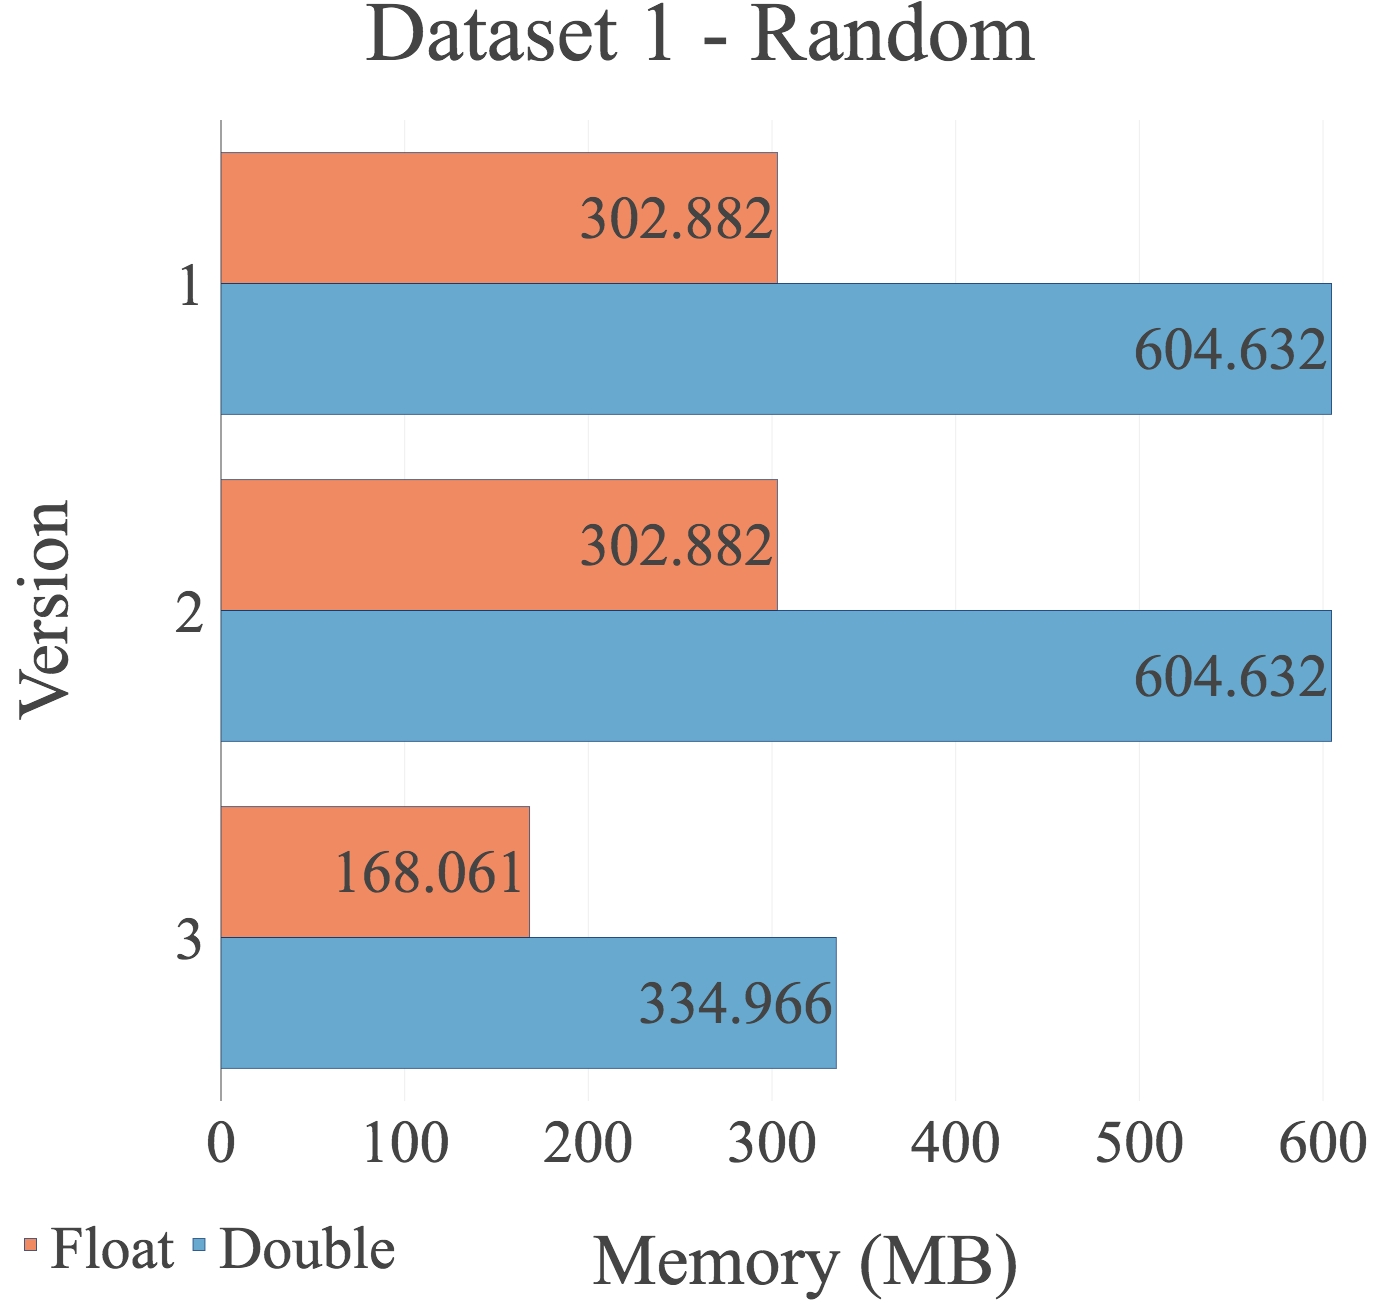
\includegraphics[width=1\linewidth]{img/experiments/mem-multi-versions-1_RAND.png}
\end{subfigure}
\begin{subfigure}{.49\textwidth}
  \centering
  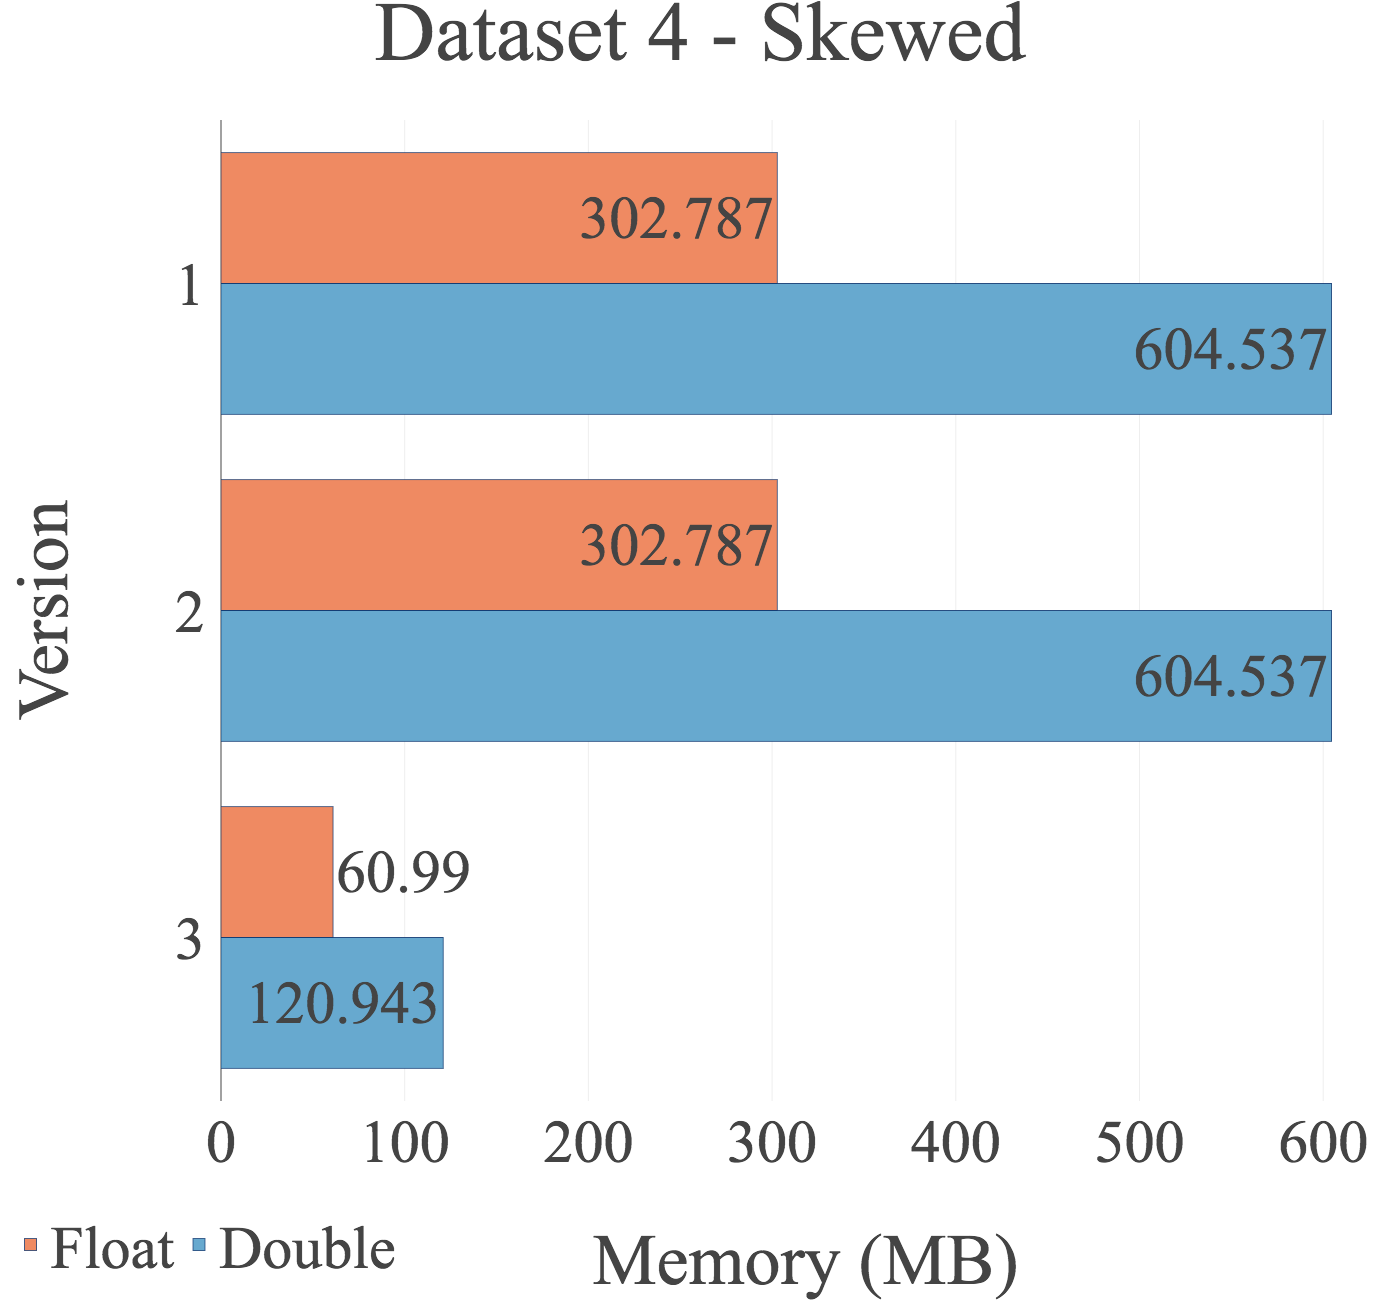
\includegraphics[width=1\linewidth]{img/experiments/mem-multi-versions-4_SKEWED.png}
\end{subfigure}
\begin{center}
  \small
  \captionof{table}{Float memory size for all 7 datasets (in MB)}
  \csvautotabular{csv/mem-multi-versions-float.csv}
\end{center}
\begin{center}
  \small
  \captionof{table}{Double memory size for all 7 datasets (in MB)}
  \csvautotabular{csv/mem-multi-versions-double.csv}
\end{center}
\caption{Memory impact of global-level padding \textit{CUDA-multi} (average global memory size)}
\label{fig:experiments:cudamulti:globalpadding}
\end{figure}

\newpage
\subsection{Sorting}
As mentioned at the end of chapter~\ref{chapter:multoptionsperthreadblock}, reducing the thread divergence on heights can be done by sorting by height, while sorting by widths can improve the options packing. We can see on fig.~\ref{fig:experiments:cudamulti:sorting}, that any sorting gives up to \textasciitilde$1.7\times$ speed-up for floats and up to \textasciitilde$1.4\times$ for doubles. The differences between sorting options is insignificant, however we can see that sorting by height often results in a slightly better speed-up. Supplementary plots in Appendix.~\ref{appendix:experiments:cudamulti:sorting} and tables in fig.~\ref{fig:experiments:cudamulti:sorting} further underline this.

As also seen in section~\ref{section:sortingcudaoption}, uniform datasets obviously do not benefit from sorting, but it has been shown that the process of sorting only slightly degrades performance.  

\begin{figure}[H]
\centering
\begin{subfigure}{.49\textwidth}
  \centering
  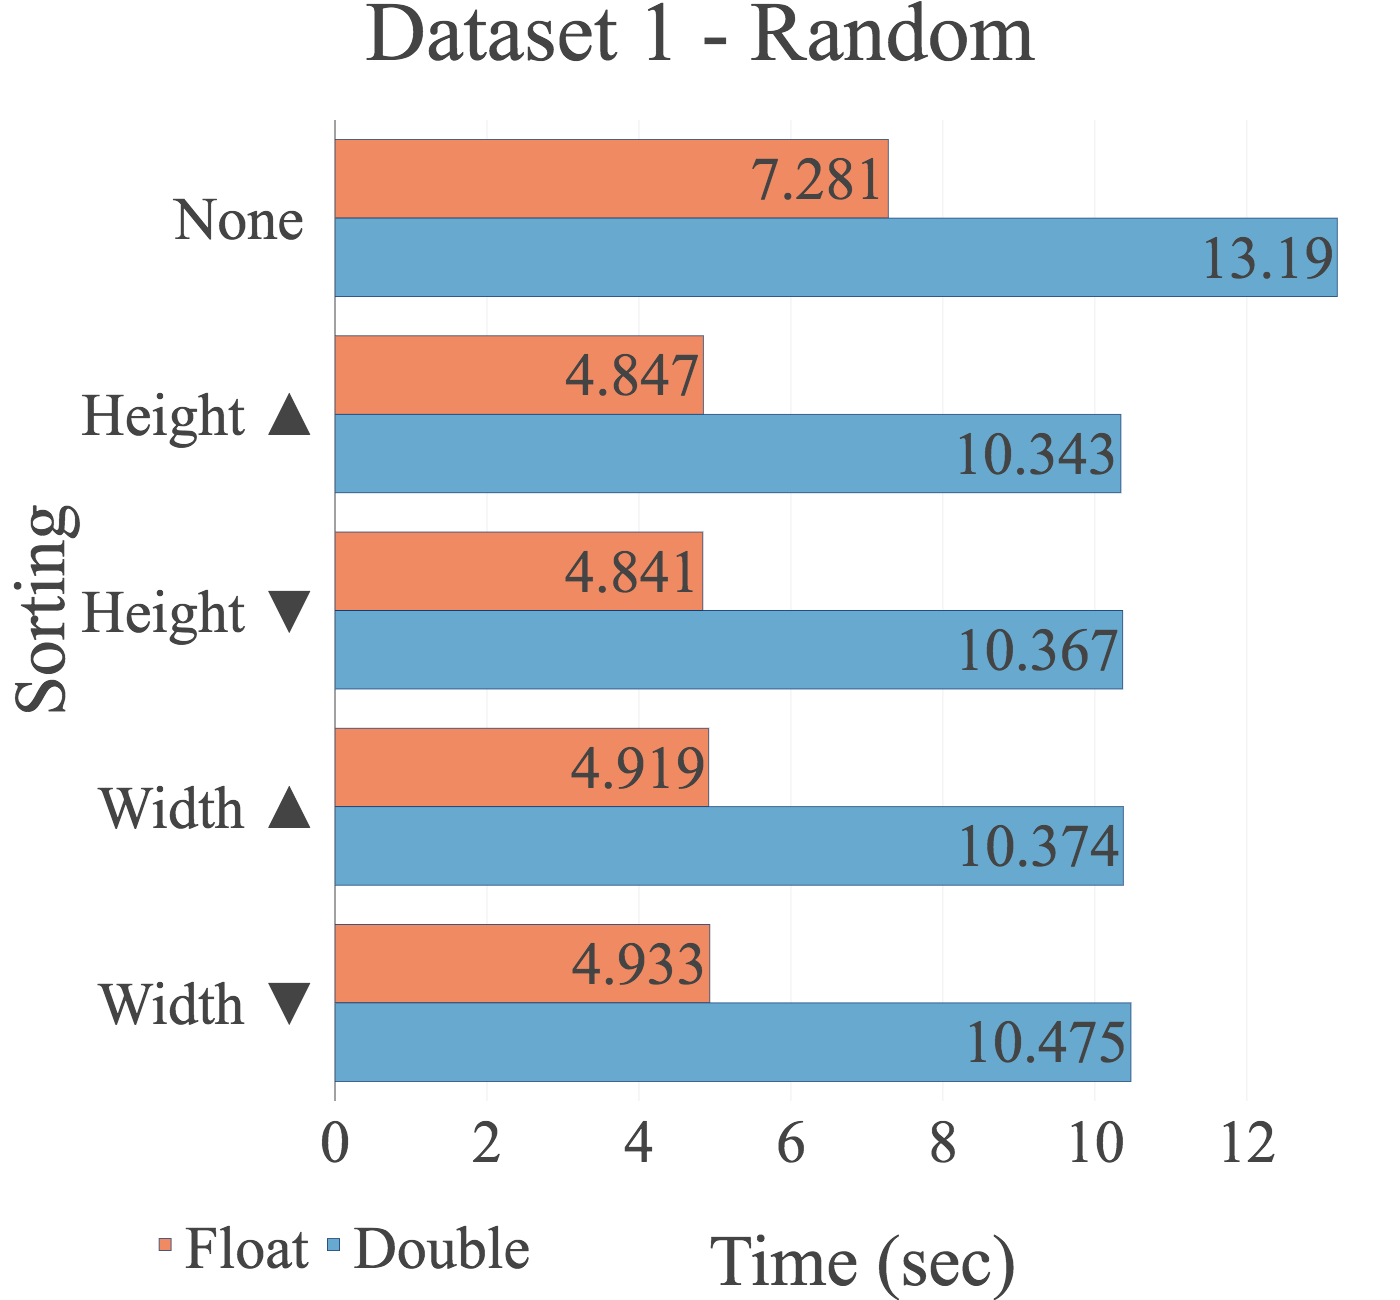
\includegraphics[width=1\linewidth]{img/experiments/multi-sorts-1_RAND.png}
\end{subfigure}
\begin{subfigure}{.49\textwidth}
  \centering
  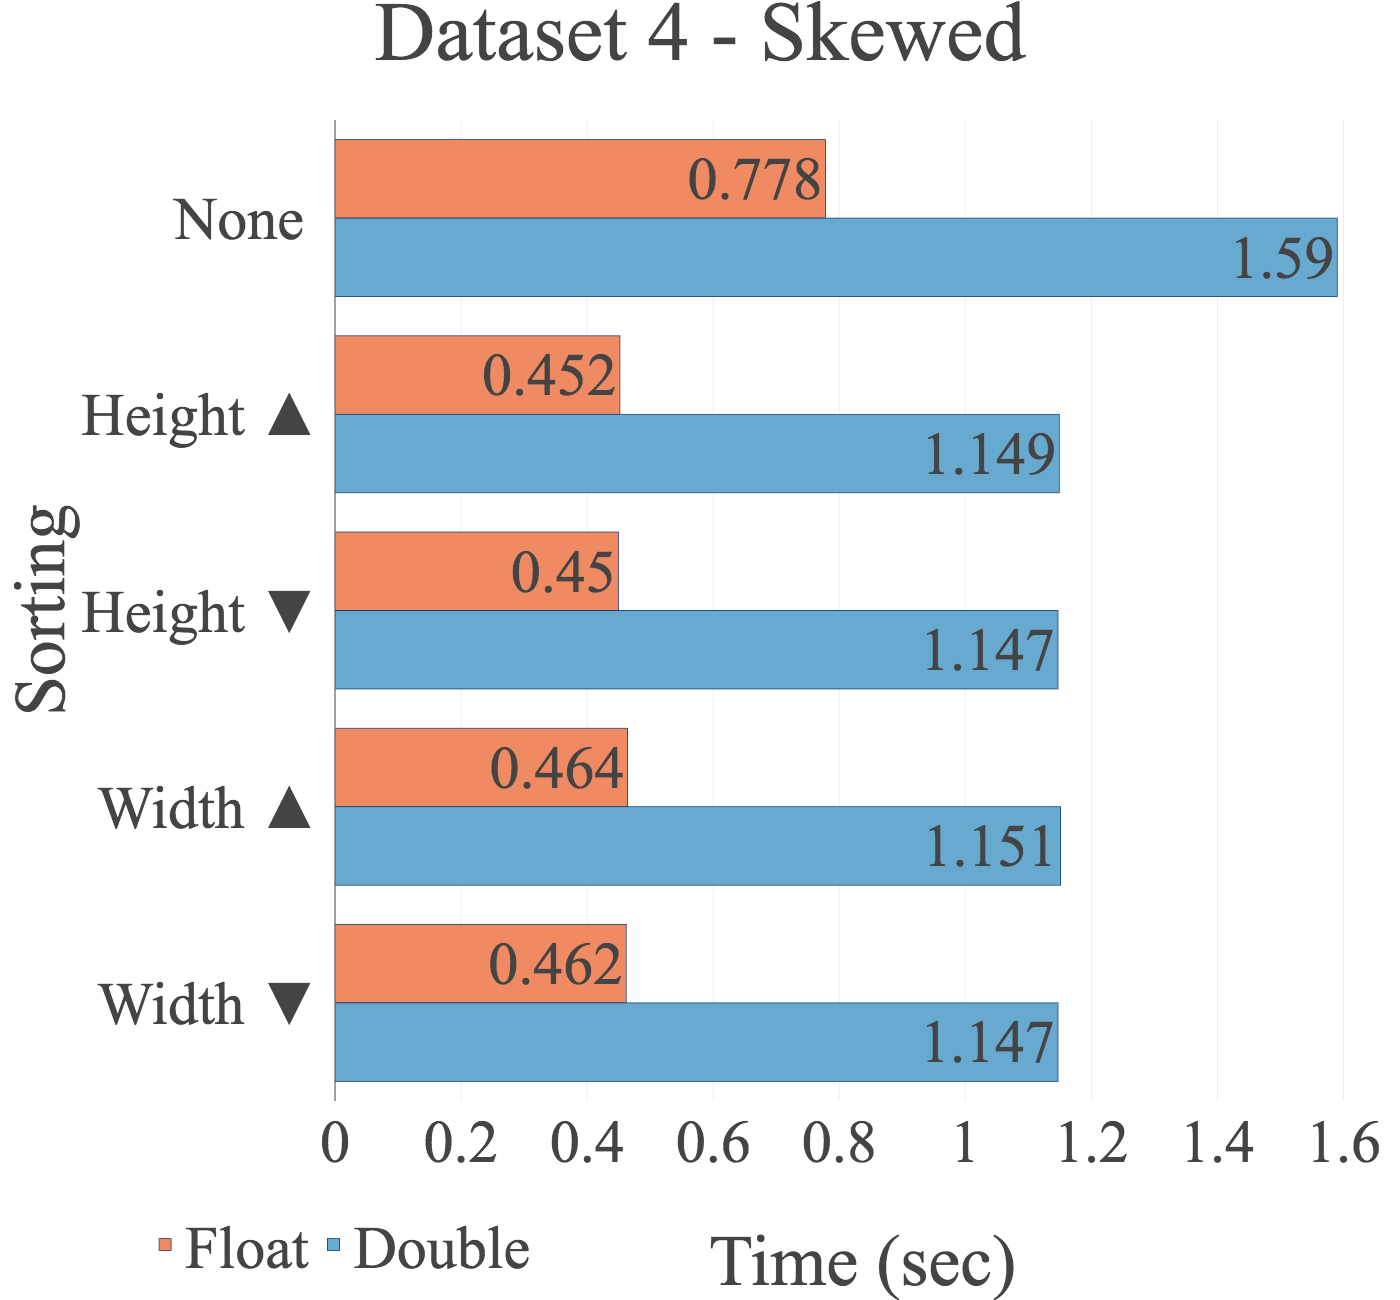
\includegraphics[width=1\linewidth]{img/experiments/multi-sorts-4_SKEWED.png}
\end{subfigure}
\begin{center}
  \small
  \captionof{table}{Float runtime for all 7 datasets (in seconds)}
  \csvautotabular{csv/multi-sorts-float.csv}
\end{center}
\begin{center}
  \small
  \captionof{table}{Double runtime for all 7 datasets (in seconds)}
  \csvautotabular{csv/multi-sorts-double.csv}
\end{center}
\caption{Performance impact of sorting padding \textit{CUDA-multi} (best runtimes)}
\label{fig:experiments:cudamulti:sorting}
\end{figure}

\newpage
\subsection{Block Sizes}
The experiments on block sizes (see fig. \ref{fig:experiments:cudamulti:blocks}) have proven that using block size of 1024 and limiting registers to 32 is always preferable, compared to using block size of 512 without limiting registers. We can see a speed-up of up to \textasciitilde$1.4\times$ on floats and \textasciitilde$1.5\times$ on doubles. Bigger block size allows packing more options in one block, while limiting the number of registers helps to achieve full occupancy on SMs, proving our performance expectations from chapter~\ref{chapter:cudamulti:optimizations}. 

\begin{figure}[H]
\centering
\begin{subfigure}{.49\textwidth}
  \centering
  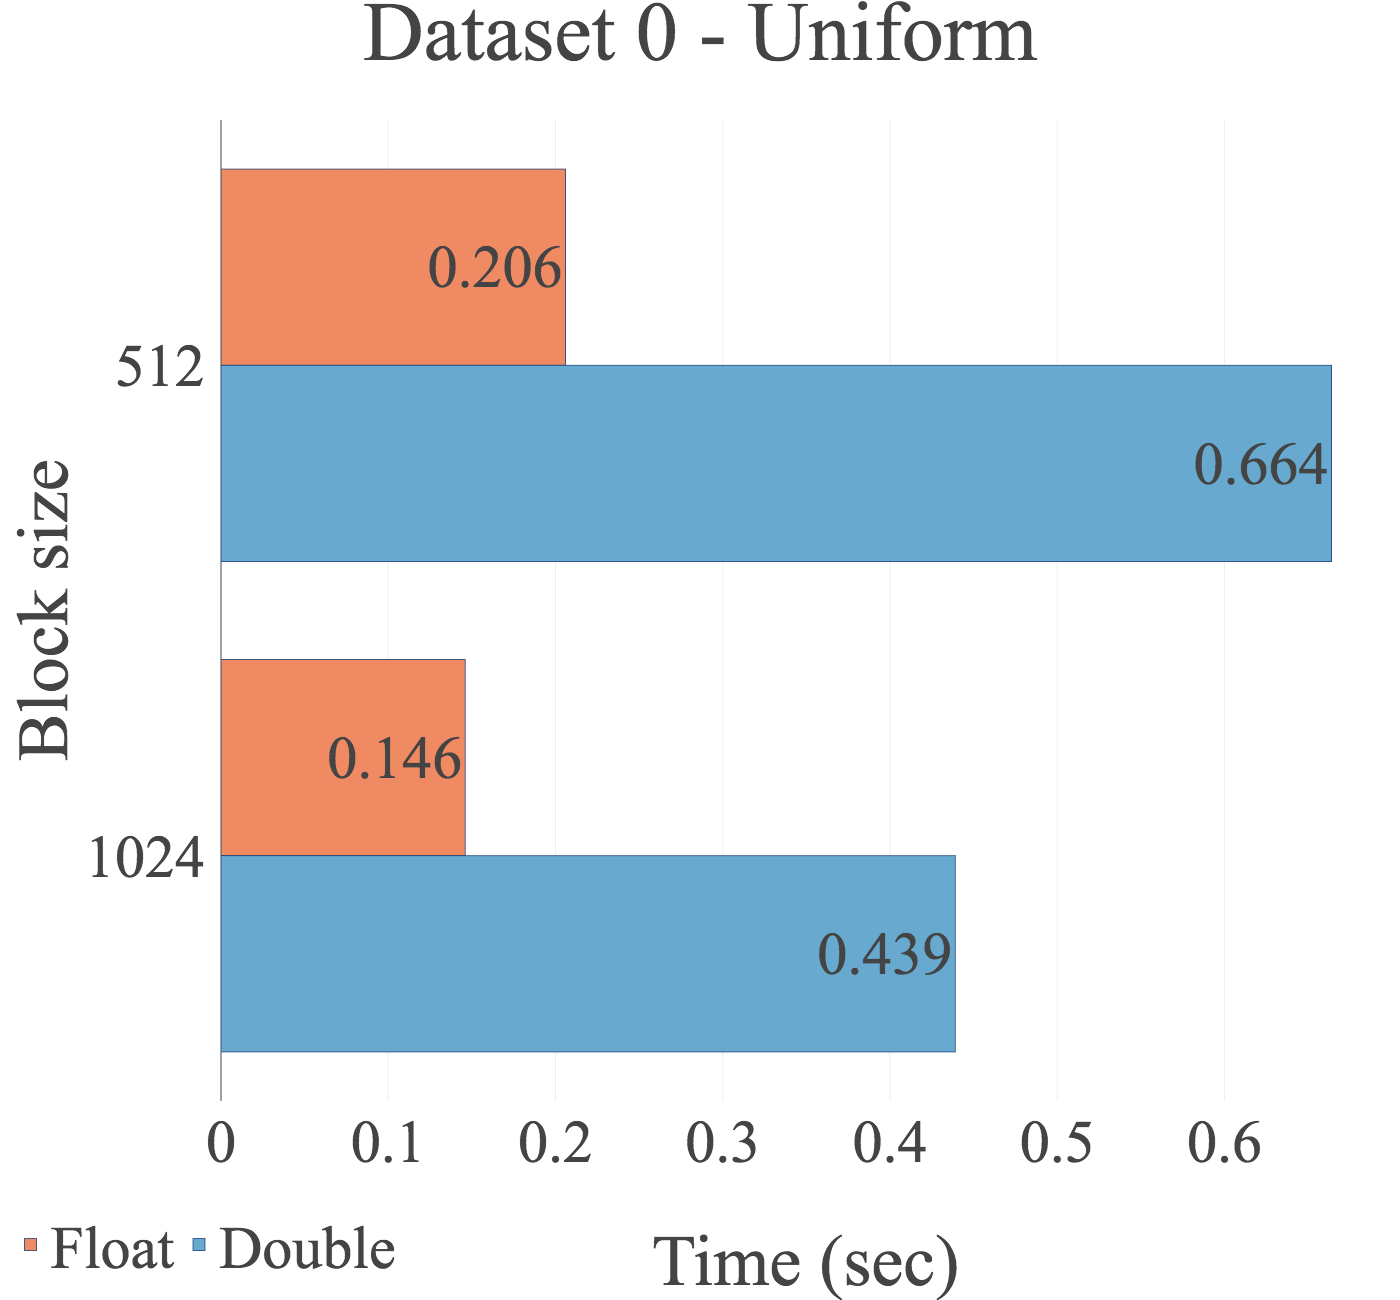
\includegraphics[width=1\linewidth]{img/experiments/multi-blocks-0_UNIFORM.png}
\end{subfigure}
\begin{subfigure}{.49\textwidth}
  \centering
  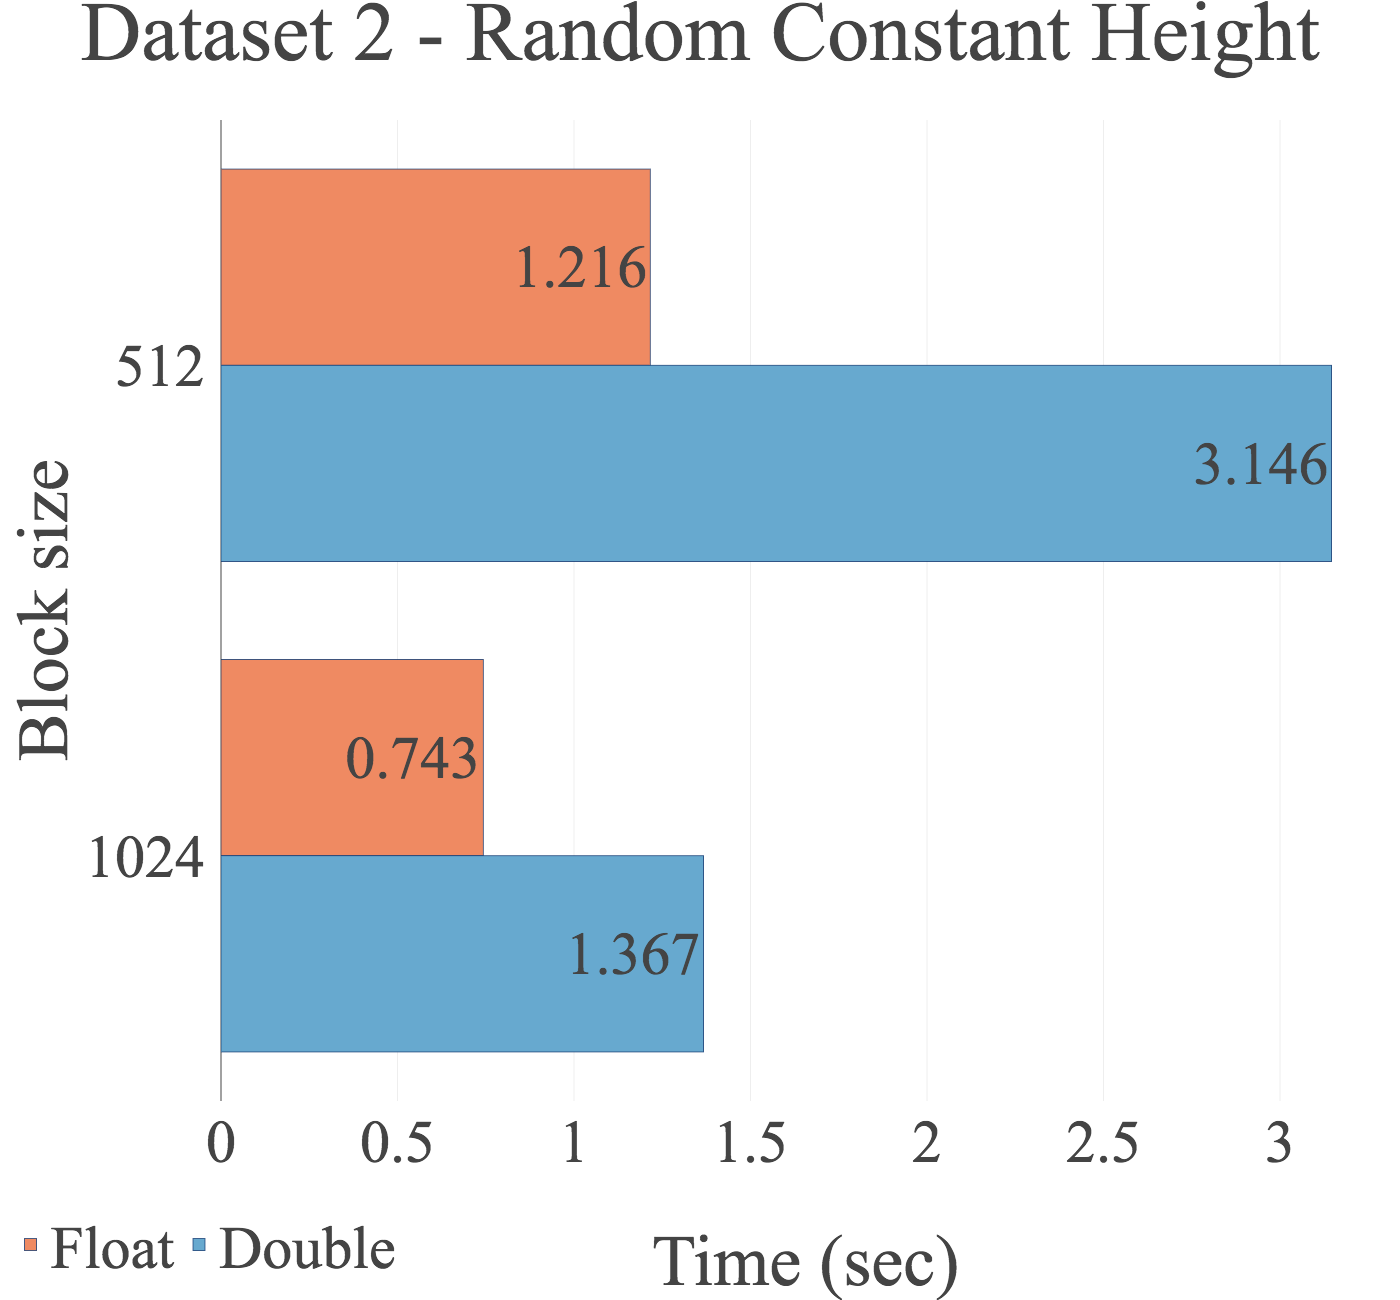
\includegraphics[width=1\linewidth]{img/experiments/multi-blocks-2_RANDCONSTHEIGHT.png}
\end{subfigure}
\begin{center}
  \small
  \captionof{table}{Float runtime for all 7 datasets (in seconds)}
  \csvautotabular{csv/multi-blocks-float.csv}
\end{center}
\begin{center}
  \small
  \captionof{table}{Double runtime for all 7 datasets (in seconds)}
  \csvautotabular{csv/multi-blocks-double.csv}
\end{center}
\caption{Performance impact of block sizes on \textit{CUDA-multi} (best runtimes)}
\label{fig:experiments:cudamulti:blocks}
\end{figure}

\newpage
\subsection{Bin Packing}
As mentioned in chapter~\ref{chapter:multoptionsperthreadblock}, in \textit{CUDA-multi}, all options are packed sequentially before invoking the kernel. Ideally, we can optimize this by implementing it in parallel. Despite that, we show on tables~\ref{table:experiments:cudamulti:sortingcostfloats} and~\ref{table:experiments:cudamulti:sortingcostdoubles} that pre-processing of the data has had insignificant impact on the performance, delaying it up to \textasciitilde$7.3$ milliseconds on average. We can also note here that (i) the times shown in the two tables show the average pre-processing time for each version (hence there may be larger runtimes than $7.3$, but still insignificant) and (ii) the runtimes include sorting too, as sorting can also have an impact on bin packing.  

\begin{figure}[H]
\begin{center}
  \small
  \captionof{table}{Float pre-processing time for all 7 datasets (in \textbf{milliseconds})}
  \csvautotabular{csv/multi-versions-prep-float.csv}
  \label{table:experiments:cudamulti:sortingcostfloats}
\end{center}
\begin{center}
  \small
  \captionof{table}{Double pre-processing time for all 7 datasets (in \textbf{milliseconds})}
  \csvautotabular{csv/multi-versions-prep-double.csv}
  \label{table:experiments:cudamulti:sortingcostdoubles}
\end{center}
\caption{Pre-processing cost in \textit{CUDA-multi} (average pre-processing times)}
\label{fig:experiments:cudamulti:prep}
\end{figure}

\newpage
\section{Parallel Speed-up}
First and foremost, we underline the performance benefits that porting code to GPGPU hardware can provide. Figures~\ref{fig:results:speedup-float} and~\ref{fig:results:speedup-double} show speed-up achieved by all parallel implementations compared to the sequential implementation, for both single (floats) and double precision respectively. Even though the sequential code could be further optimized, it does already provide a useful metric for comparing datasets with different workloads. As it can be seen, \textit{CUDA-option} is the principal winner of this comparison, with speed-ups up to \textasciitilde$529\times$ faster than the sequential implementation on floats and up to \textasciitilde$87\times$ faster on doubles. \textit{CUDA-multi} prevails on dataset 4 - Skewed with a speed-up of \textasciitilde$161\times$ on floats and \textasciitilde$54\times$ on doubles. 

% From introduction:
% It still holds that sequentializing the inner-parallelism in excess (to the ones needed to saturate hardware) is the right thing to do when the divergence is randomly distributed --- even though this method necessarily leaves one level of divergence unoptimized. However, when the distribution of divergence is skewed on both levels, it is better to exploit all parallelism because this allows to optimize all divergence.

Here we find out that if the data distribution is \underline{skewed on both heights and widths}, it is better to \underline{exploit both levels of parallelism} because this allows to further optimize thread divergence. This feature of the dataset can easily be computed using the \textbf{skewness} statistical measure. Dataset 4 - Skewed has $2.40$ skewness on heights and $5.19$ on widths (as seen in Appendix~\ref{appendix:data:skewed}), in contrast with other datasets that have skewness close to zero on heights or widths or both.

Additionally, the experiments we have performed on smaller datasets\footnote{Even more experiments can be seen in Appendix~\ref{appendix:experiments:implementations}} (see fig.~\ref{fig:results:speedup-float-small} and~\ref{fig:results:speedup-double-small}) have exposed that \textit{CUDA-multi} outperforms \textit{CUDA-option} up to \textasciitilde$13\times$ in runtime when the datasets are small enough. Furthermore we can see that the performance of \textit{CUDA-option} and \textit{Futhark-basic} increases with the number of options, while \textit{CUDA-multi} is not affected by it. This leads us to believe that there exists a certain threshold for each data distribution, which can be used to dynamically switch between \textit{CUDA-multi} and \textit{CUDA-option} for optimal performance.    

\begin{figure}[H]
	\centering
	\caption{Comparisons of parallel speed-ups over sequential implementation using single precision. CUDA-option is faster on all datasets except 4 - Skewed, where CUDA-multi is faster.}
    \label{fig:results:speedup-float}
    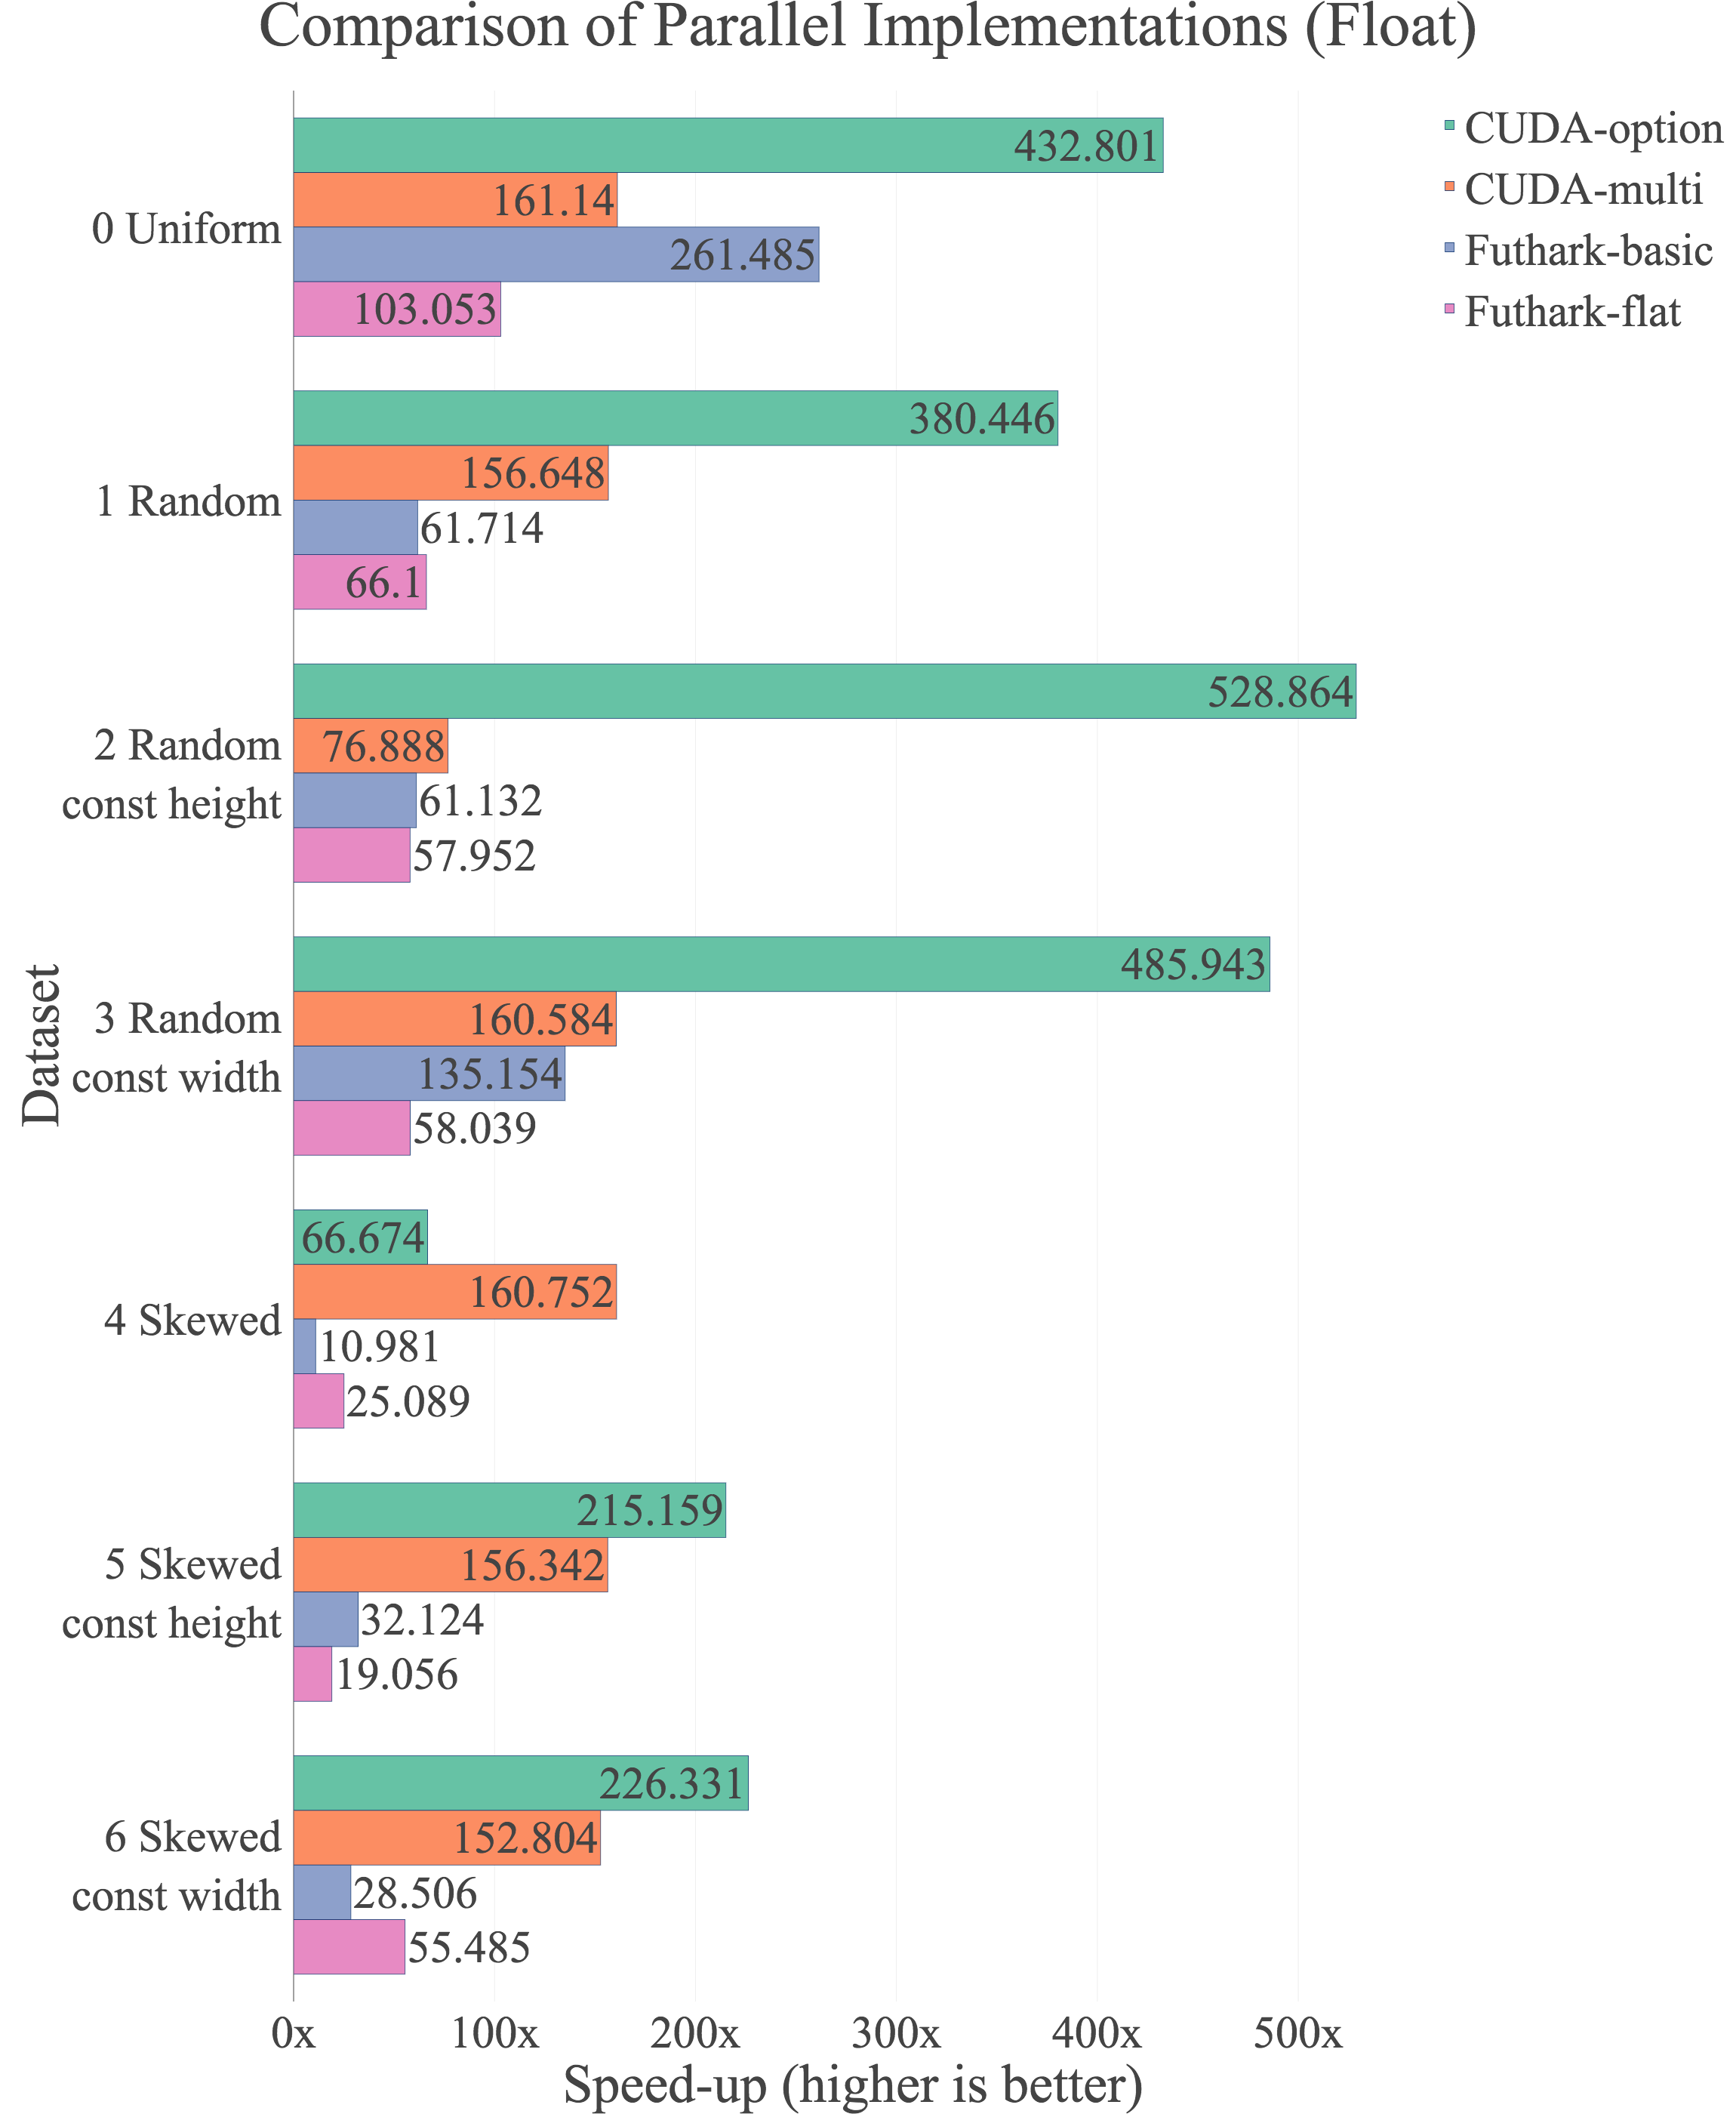
\includegraphics[width=1\textwidth]{img/experiments/all-approaches-float.png}
\end{figure}

\begin{figure}[H]
	\centering
	\caption{Comparisons of parallel speed-ups over sequential implementation using double precision. CUDA-option is faster on all datasets except 4 Skewed, where CUDA-multi is faster.}
    \label{fig:results:speedup-double}
    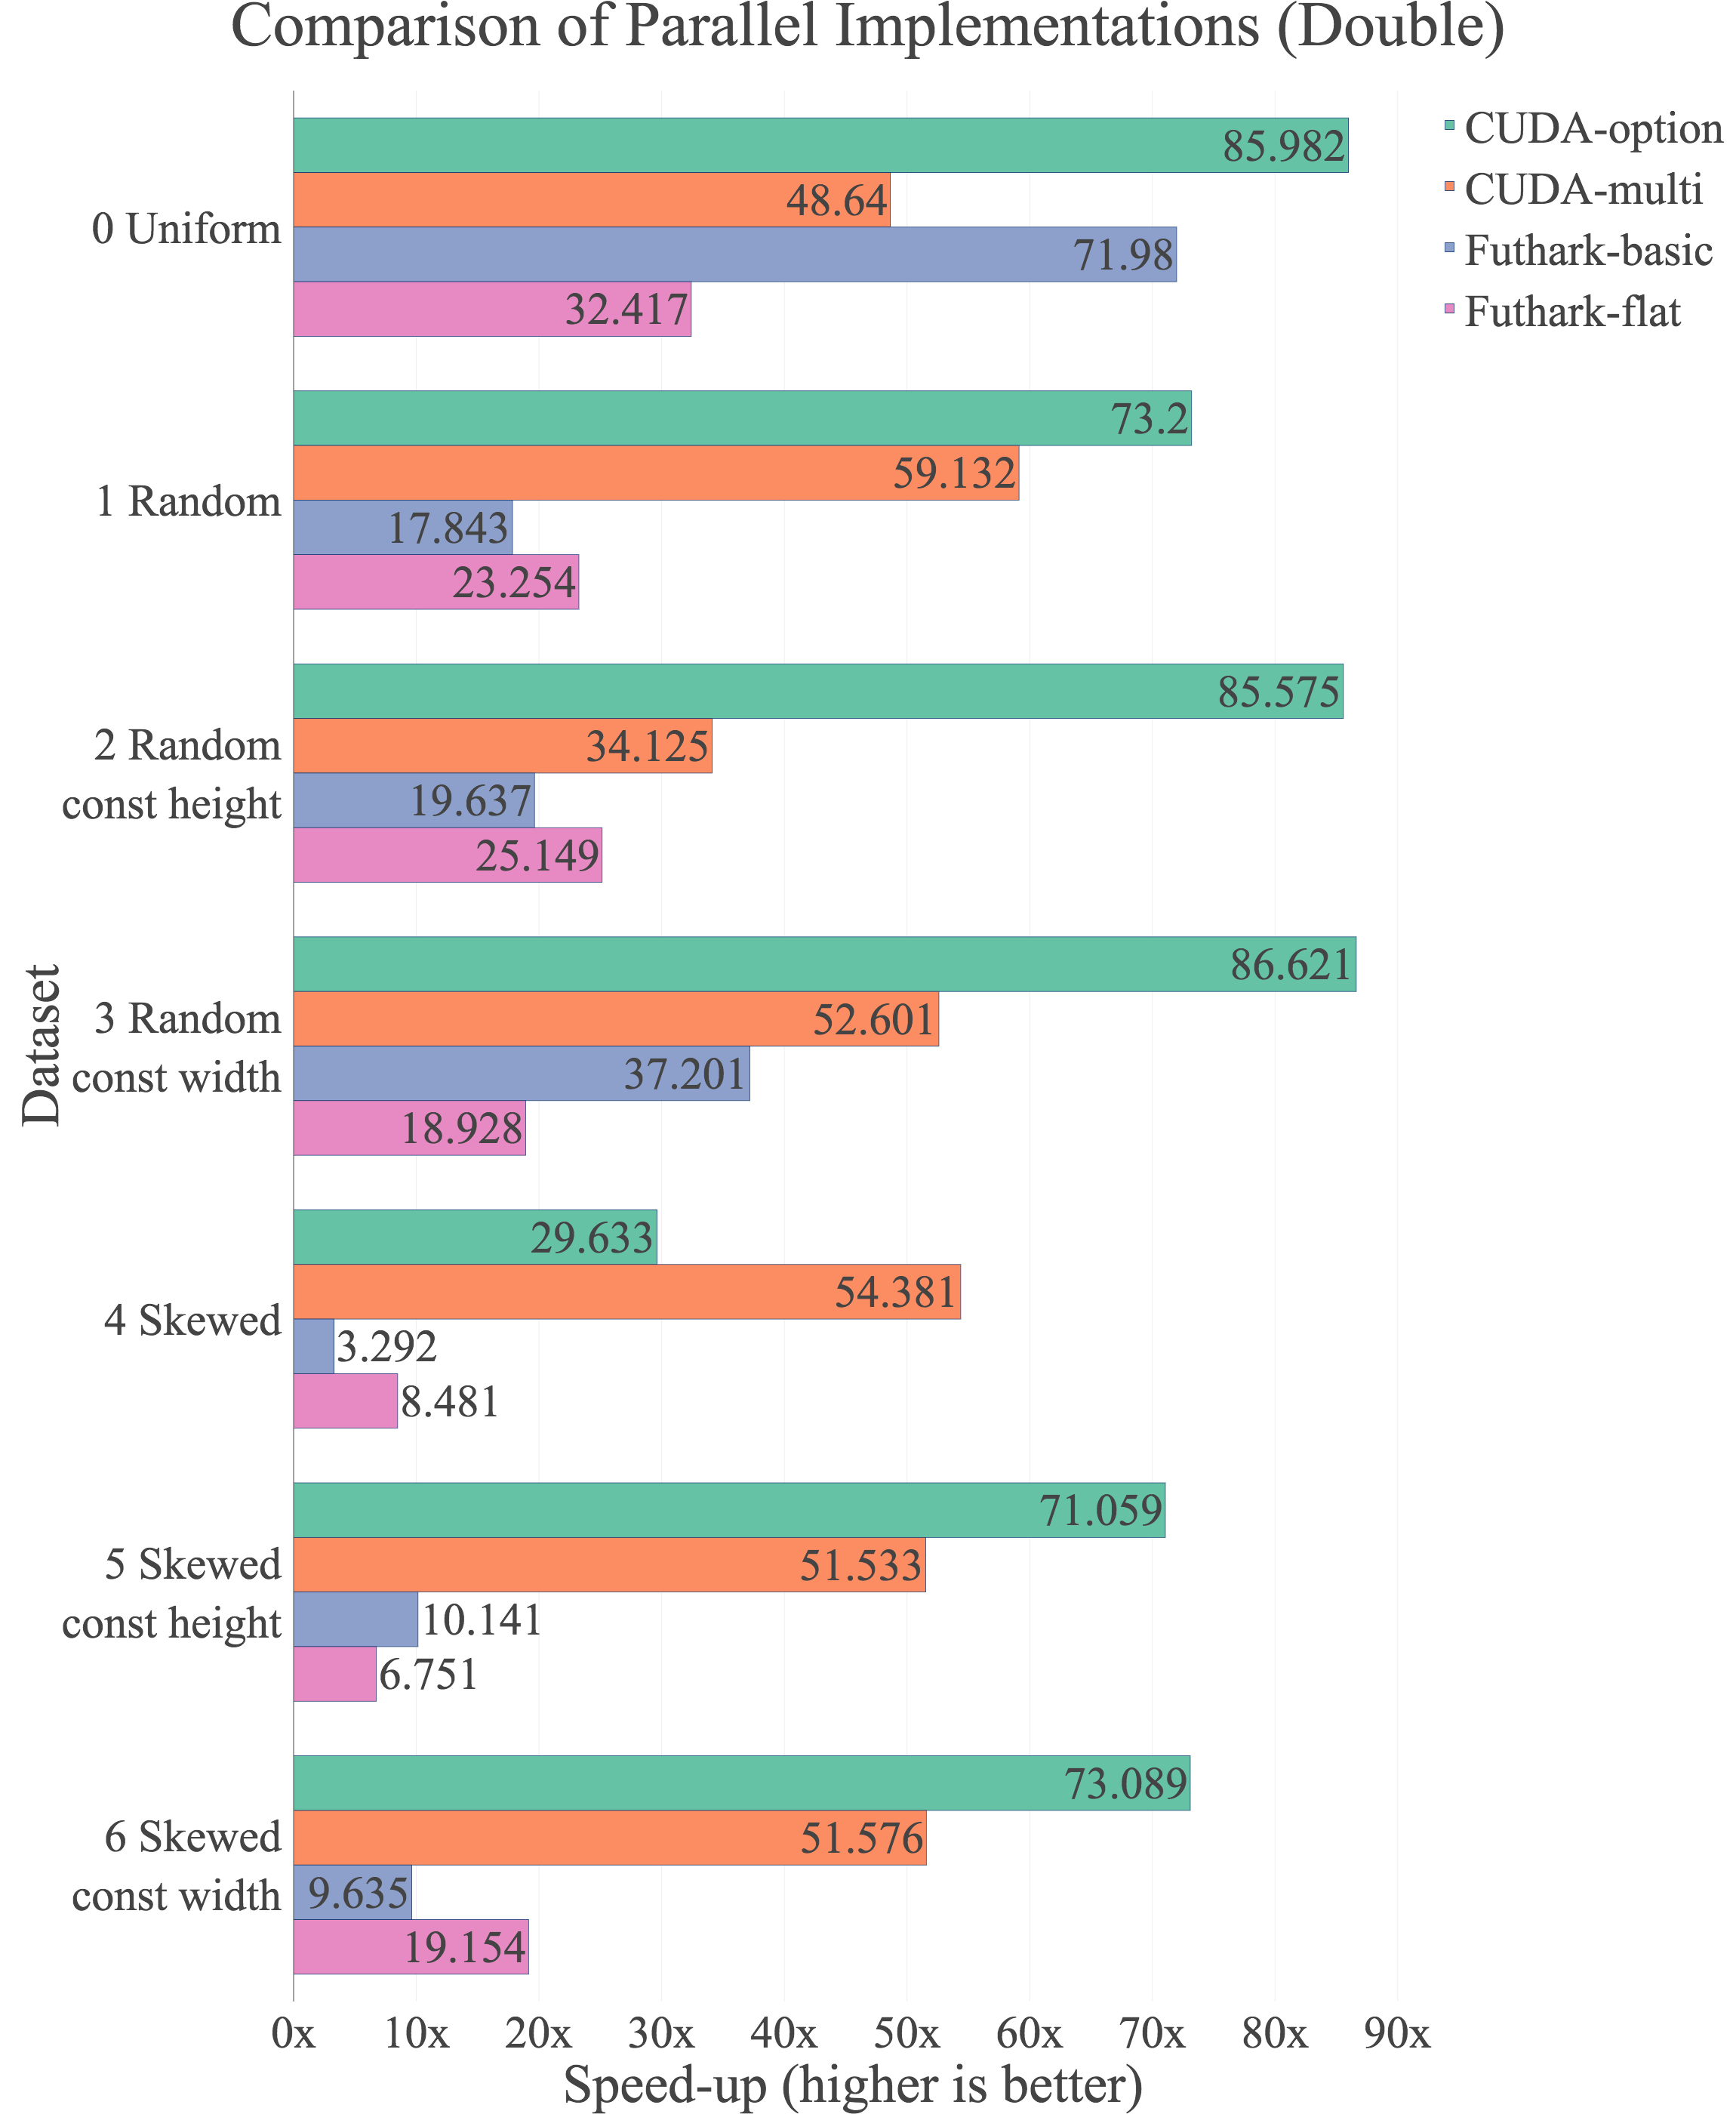
\includegraphics[width=1\textwidth]{img/experiments/all-approaches-double.png}
\end{figure}

\begin{figure}[H]
	\centering
	\caption{Comparisons of parallel speed-ups on smaller datasets over sequential implementation using single precision.}
    \label{fig:results:speedup-float-small}
    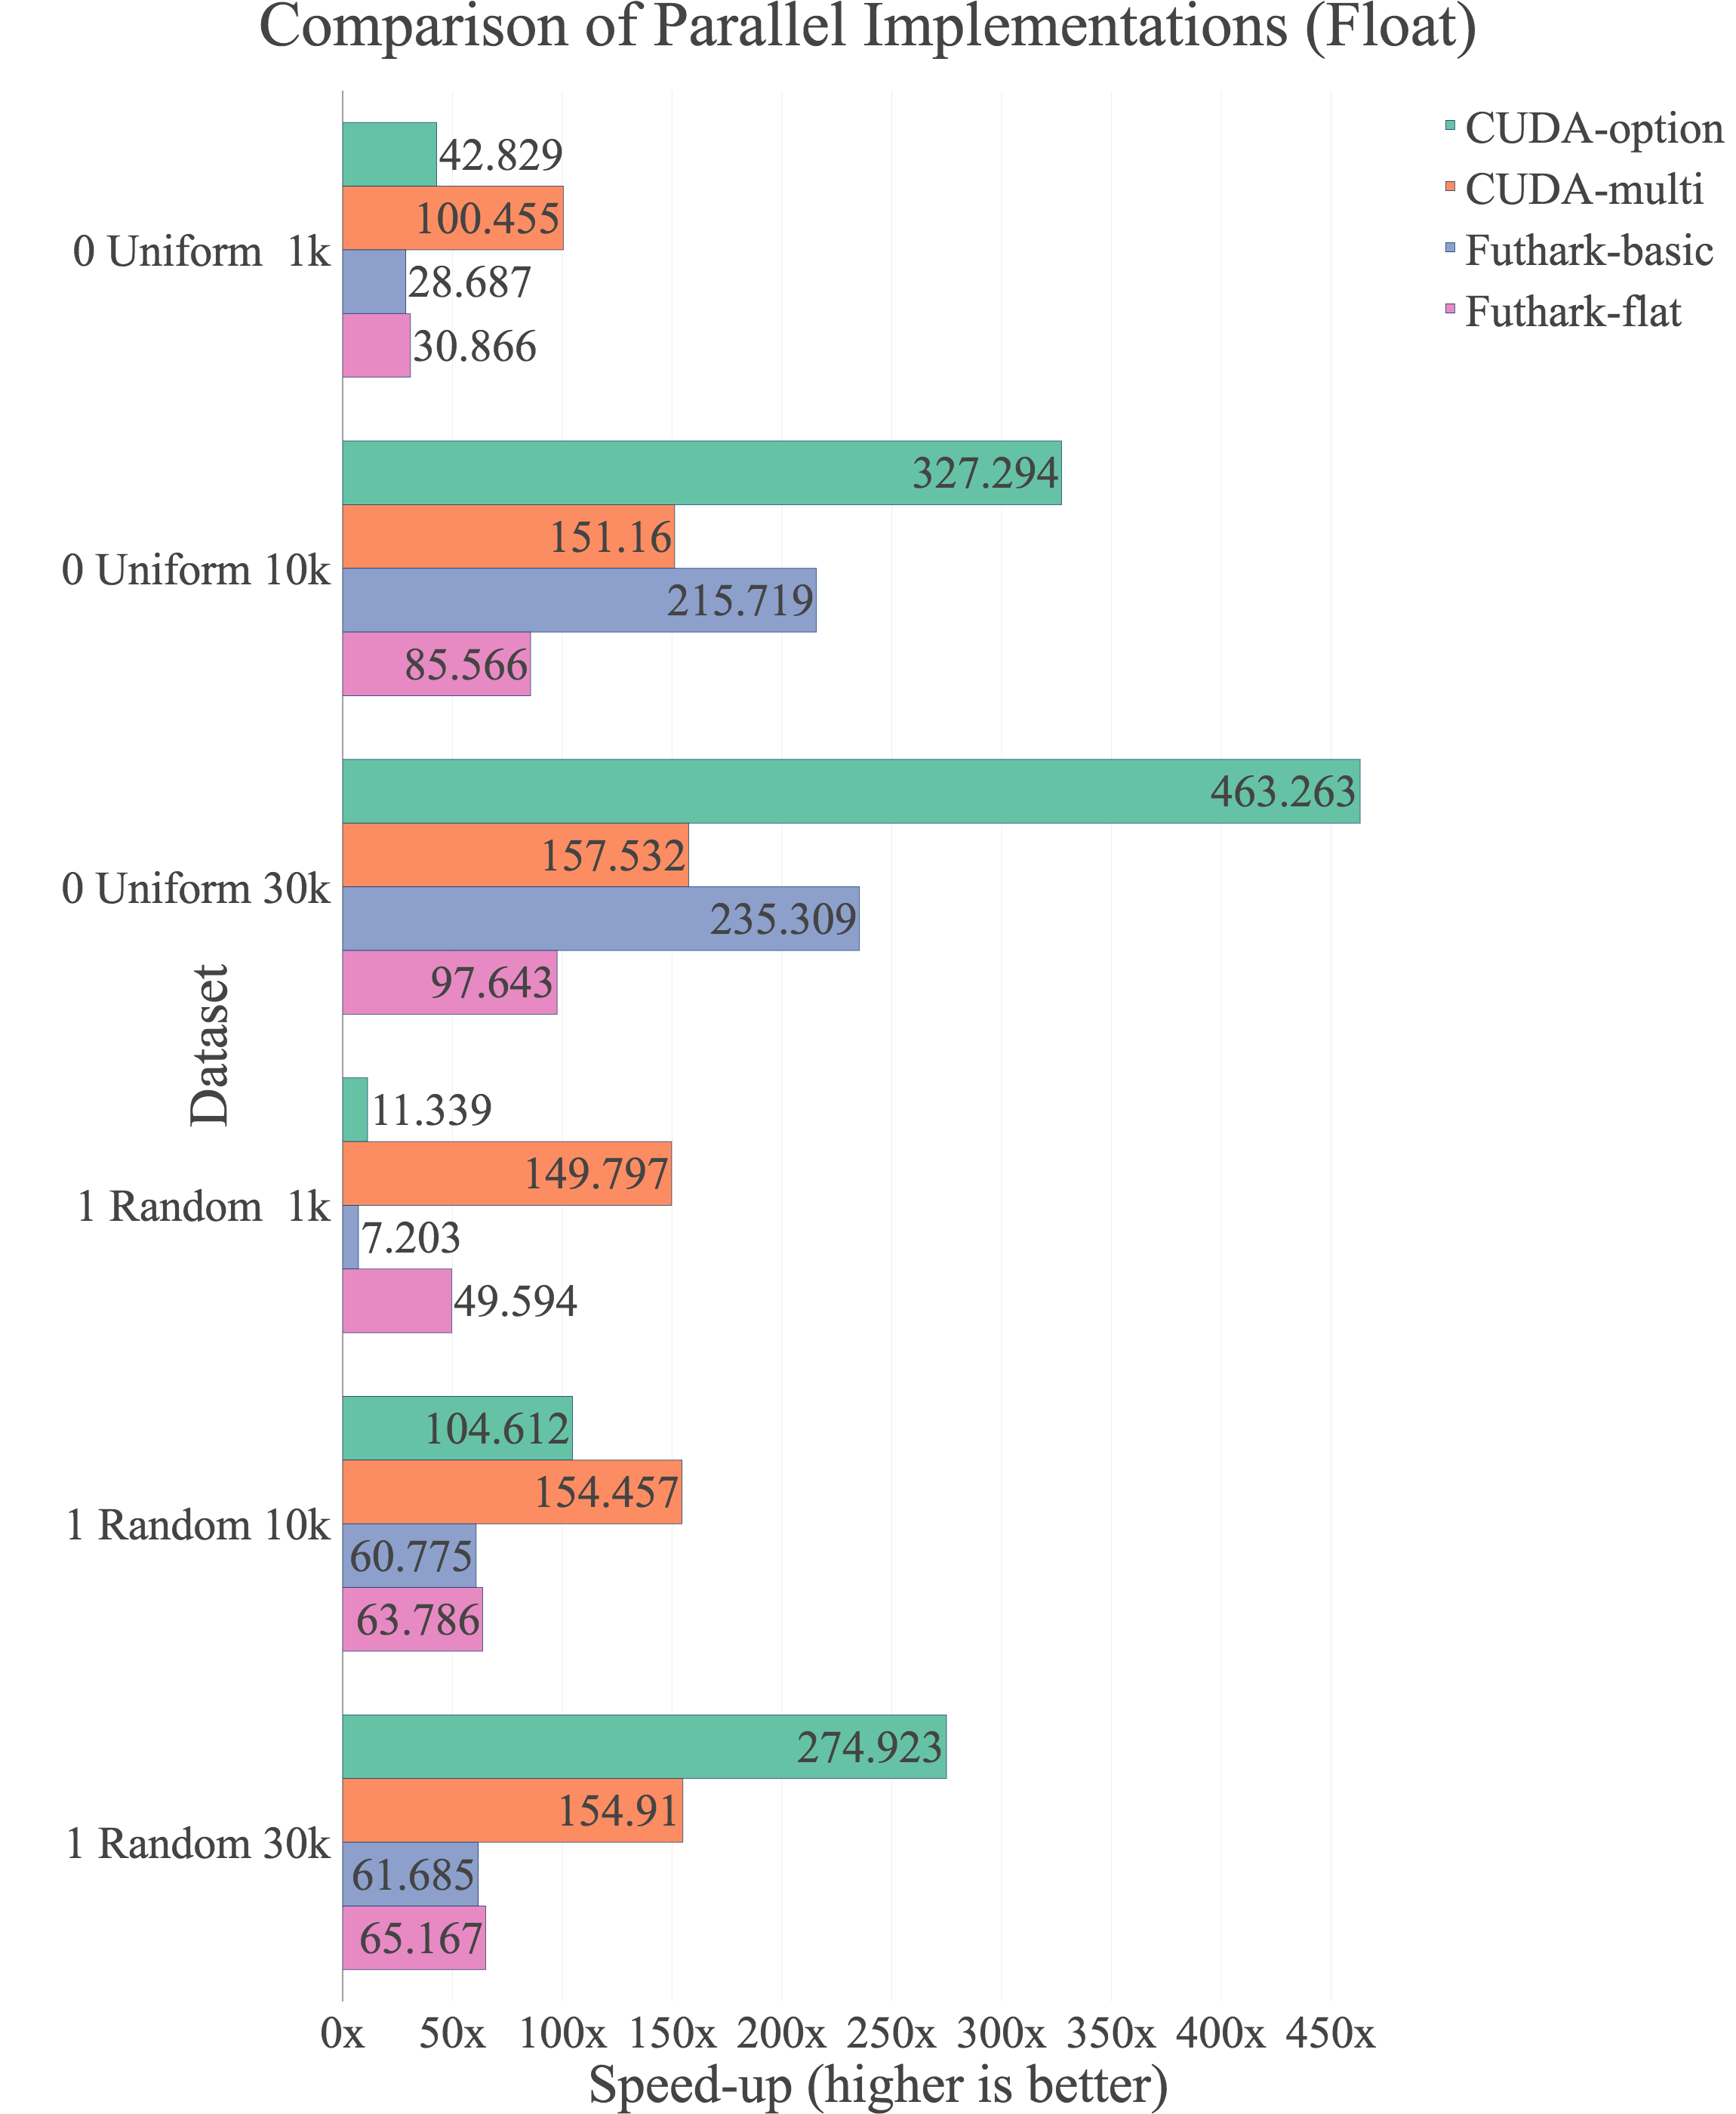
\includegraphics[width=1\textwidth]{img/experiments/small-text-approaches-float.png}
\end{figure}

\begin{figure}[H]
	\centering
	\caption{Comparisons of parallel speed-ups on smaller datasets over sequential implementation using double precision.}
    \label{fig:results:speedup-double-small}
    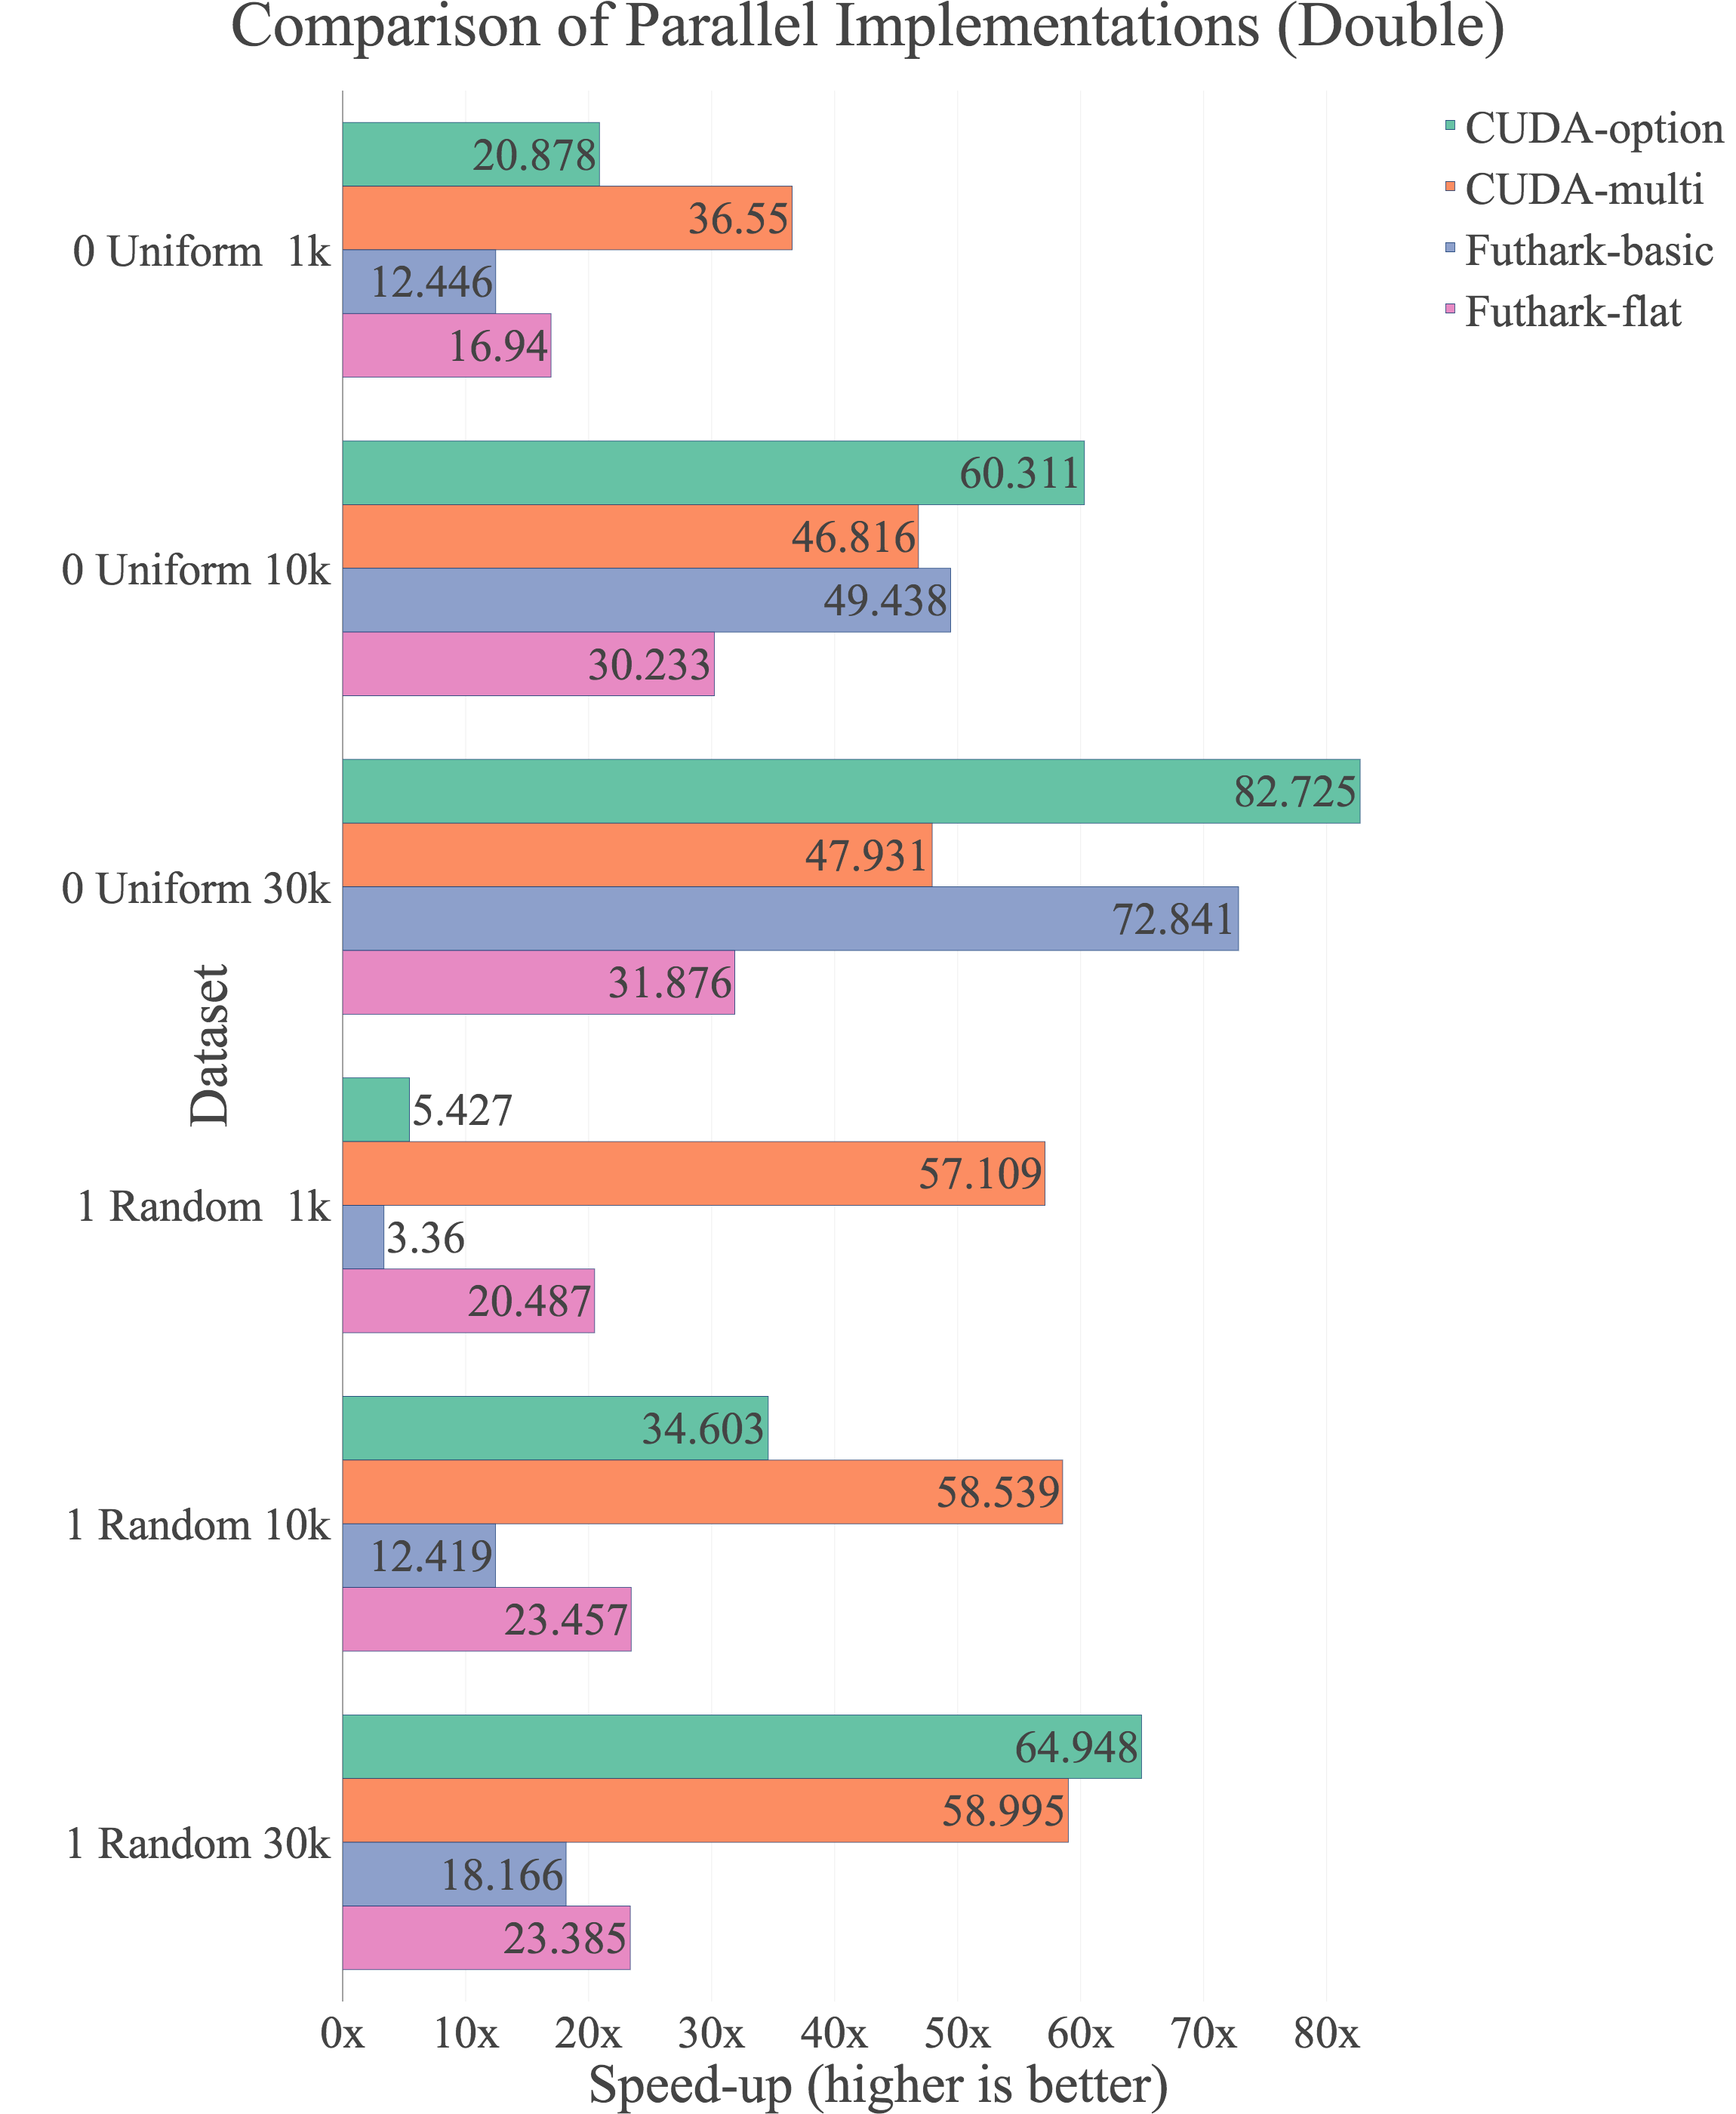
\includegraphics[width=1\textwidth]{img/experiments/small-text-approaches-double.png}
\end{figure}

\section{Key findings}
The experiments have shown that:
\begin{itemize}
    \item Memory coalescing has positive impact on the runtime performance of \textit{CUDA-option}, at the cost of higher memory consumption. It is therefore important to optimize the global arrays and reduce their padding as much as possible. Coalescing on \textit{CUDA-multi} on the other hand did not appear to be as effective but more granular padding has shown performance gains, most probably because of improved locality of reference (caching).    
    
    \item Sorting has shown positive performance impact on both \textit{CUDA-option} and \textit{CUDA-multi} runtimes at neglectable runtime costs. An exception can be found when the data distribution is uniform, and consists of the same option replicated many times. However, this seems highly impractical in real life situations and can be easily detected. In terms of choosing the order, descending sorting by both width and height has shown the best results, but we have also shown that the correct choice is mostly dependent on the data. 
    
    \item Choosing the correct block sizes has also shown to produce significant runtime impact on \textit{CUDA-option}. However, this is also dependent on the data distribution, as skewed datasets tend to benefit more from larger block sizes, such as 256 and 512, while uniform and random datasets tend to have highest performance with block size of 128. For \textit{CUDA-multi}, it is best to chose block size 1024 to pack in as many options as possible, while limiting the number of registers to 32 to achieve full occupancy of SMs.
    
    \item In terms of runtime, \textit{CUDA-option} has been dominant on all datasets except 4 - Skewed, where \textit{CUDA-multi} wins by almost a double margin. This discovery underlines the statement that parallel optimization is often sensitive to the dataset, hence it is important to explore the impacts of different degrees of parallelism. Furthermore, this allows the use of dynamic analysis in order to determine the optimal strategy for each dataset. 
    
    \item There exists a certain threshold for the number of options in each data distribution, which can be used to dynamically choose \textit{CUDA-multi} over \textit{CUDA-option} if the dataset has small enough number of options.  
\end{itemize} 

Another interesting finding of less relevance to the thesis is that the sequential implementation is on average 15\% faster with \underline{doubles} than with floats (can be seen on the figures in Appendix~\ref{appendix:experiments:implementations}). In all our parallel implementations, \underline{float} achieves 2 to $6\times$ higher speed-ups than double. This difference can be explained with the fact that double precision (taking twice the memory) is much heavier on registers and cache which are more complex on the CPU cores than on the GPU's CUDA cores. 

\section*{Summary}
This chapter has shown the experiments we have performed to put our implementations to the test. It has introduced the impacts of the optimizations we have done, both in terms of runtime and memory consumption. Later in this chapter we have shown a comparison of all implementations, which has also led to the most important discovery - that \textit{CUDA-multi} can show speed-up over \textit{CUDA-option} on some datasets. Additionally, we describe all key findings of our experiments in the end of the chapter, with the idea of drawing meaningful conclusions later in the thesis. The next chapter will introduce related work on the topic, leading up to our conclusions, which will follow right after.